\documentclass[12pt, a4paper]{article}
\usepackage[utf8]{inputenc}
\usepackage{geometry}
\usepackage{graphicx}
\usepackage{multicol}
\usepackage{multirow}
\usepackage{tikz}
\usepackage{tabularx}
\usepackage{float}
\usepackage{array,booktabs,ragged2e}
 \usepackage{amsmath}
\usepackage{siunitx}
\usepackage{physics}
\usepackage{xcolor}
\usepackage{wasysym}
\usepackage{ulem} %tallymarks
\usepackage{xkeyval}



\geometry{top=2.5cm, bottom=1.25cm, left=1.5cm, right=1.5cm}


%-----------------------------------------------------------
% 4 OPTION ON RIGHT MCQ WITH IMAGE ON LEFT
%-----------------------------------------------------------

% DEFINE KEY FOR mcqfourimg %

\makeatletter
\define@key{mcqfourimg}{questionnumber}{\def\mcqquestion{#1}}
\define@key{mcqfourimg}{questiontext}{\def\mcqquestiontext{#1}}
\define@key{mcqfourimg}{imgwidth}{\def\mcqimgwidth{#1}}
\define@key{mcqfourimg}{imgheight}{\def\mcqimgheight{#1}}
\define@key{mcqfourimg}{img}{\def\mcqimg{#1}}
\define@key{mcqfourimg}{optionA}{\def\mcqoptionA{#1}}
\define@key{mcqfourimg}{optionB}{\def\mcqoptionB{#1}}
\define@key{mcqfourimg}{optionC}{\def\mcqoptionC{#1}}
\define@key{mcqfourimg}{optionD}{\def\mcqoptionD{#1}}
\define@key{mcqfourimg}{questionTag}{\def\mcqquestionTag{#1}}
\define@key{mcqfourimg}{correctoption}{\def\mcqcorrectoption{#1}}
\define@key{mcqfourimg}{leftmini}{\def\mcqleftmini{#1}}
\define@key{mcqfourimg}{rightmini}{\def\mcqrightmini{#1}}

% COMMAND FOR mcqfourimg %

\newcommand{\mcqfourimg}[1]{%
  \setkeys{mcqfourimg}{#1}%
  \vspace{1.5mm}
  \begin{raggedright}
    \textbf{Question Tag:} \mcqquestionTag \hfill \textbf{Correct Option:} \mcqcorrectoption\\
  \end{raggedright}
  \vspace{\baselineskip}
  \begin{raggedright}
    \textbf{Question \mcqquestion:} \mcqquestiontext\\
    \medskip
  \end{raggedright}
  \begin{minipage}[]{\mcqleftmini\linewidth}
    \includegraphics[width=\mcqimgwidth, height=\mcqimgheight]{\mcqimg}
  \end{minipage}\hfill
  \begin{minipage}[]{\mcqrightmini\linewidth}
      (a) \medskip \mcqoptionA\\
      (b) \medskip \mcqoptionB\\
      (c) \medskip \mcqoptionC\\
      (d) \medskip \mcqoptionD\\
   \end{minipage}
  \vspace{5mm}
}

%-----------------------------------------------------------
% 4 OPTION MCQ SEPARATED IN 2 COLS
%-----------------------------------------------------------

% DEFINE KEY FOR mcqfourtwo %

\define@key{mcqfourtwo}{questionnumber}{\def\mcqfourtwoquestion{#1}}
\define@key{mcqfourtwo}{questiontext}{\def\mcqfourtwoquestiontext{#1}}
\define@key{mcqfourtwo}{optionA}{\def\mcqfourtwooptionA{#1}}
\define@key{mcqfourtwo}{optionB}{\def\mcqfourtwooptionB{#1}}
\define@key{mcqfourtwo}{optionC}{\def\mcqfourtwooptionC{#1}}
\define@key{mcqfourtwo}{optionD}{\def\mcqfourtwooptionD{#1}}
\define@key{mcqfourtwo}{questionTag}{\def\mcqfourtwoquestionTag{#1}}
\define@key{mcqfourtwo}{correctoption}{\def\mcqfourtwocorrectoption{#1}}

% COMMAND FOR mcqfourtwo %

\newcommand{\mcqfourtwo}[1]{%
  \setkeys{mcqfourtwo}{#1}%
  \vspace{1.5mm}
  \begin{raggedright}
    \textbf{Question Tag:} \mcqfourtwoquestionTag \hfill \textbf{Correct Option:} \mcqfourtwocorrectoption\\
  \end{raggedright}
  \vspace{\baselineskip}
  \begin{raggedright}
    \textbf{Question \mcqfourtwoquestion:} \mcqfourtwoquestiontext\\
    \begin{multicols}{2}
      (a) \medskip \mcqfourtwooptionA\\
      (c) \medskip \mcqfourtwooptionC\\
      \columnbreak
      (b) \medskip \mcqfourtwooptionB\\
      (d) \medskip \mcqfourtwooptionD\\
    \end{multicols}
  \end{raggedright}
  \vspace{5mm}
}

%-----------------------------------------------------------
% 2 OPTION MCQ SEPARATED IN 2 COLS
%-----------------------------------------------------------

% DEFINE KEY FOR mcqtwotwo %

\define@key{mcqtwotwo}{questionnumber}{\def\mcqtwotwoquestion{#1}}
\define@key{mcqtwotwo}{questiontext}{\def\mcqtwotwoquestiontext{#1}}
\define@key{mcqtwotwo}{optionA}{\def\mcqtwotwooptionA{#1}}
\define@key{mcqtwotwo}{optionB}{\def\mcqtwotwooptionB{#1}}
\define@key{mcqtwotwo}{questionTag}{\def\mcqtwotwoquestionTag{#1}}
\define@key{mcqtwotwo}{correctoption}{\def\mcqtwotwocorrectoption{#1}}

% COMMAND FOR mcqtwotwo %

\newcommand{\mcqtwotwo}[1]{%
  \setkeys{mcqtwotwo}{#1}%
  \vspace{2.5mm}
  \begin{raggedright}
    \textbf{Question Tag:} \mcqtwotwoquestionTag \hfill \textbf{Correct Option:} \mcqtwotwocorrectoption\\
  \end{raggedright}
  \vspace{\baselineskip}
  \begin{raggedright}
    \textbf{Question \mcqtwotwoquestion:} \mcqtwotwoquestiontext\\
    \begin{multicols}{2}
      (a) \medskip \mcqtwotwooptionA\\
      (b) \medskip \mcqtwotwooptionB\\
    \end{multicols}
  \end{raggedright}
}


%-----------------------------------------------------------
%              4 OPTION MCQ SEPARATED IN 4 COLS
%-----------------------------------------------------------

% DEFINE KEY FOR mcqfourfour %

\define@key{mcqfourfour}{questionnumber}{\def\mcqfourfourquestionnumber{#1}} 
\define@key{mcqfourfour}{questiontext}{\def\mcqfourfourquestiontext{#1}}
\define@key{mcqfourfour}{optionA}{\def\mcqfourfouroptionA{#1}}
\define@key{mcqfourfour}{optionB}{\def\mcqfourfouroptionB{#1}}
\define@key{mcqfourfour}{optionC}{\def\mcqfourfouroptionC{#1}}
\define@key{mcqfourfour}{optionD}{\def\mcqfourfouroptionD{#1}}
\define@key{mcqfourfour}{questionTag}{\def\mcqfourfourquestionTag{#1}} 
\define@key{mcqfourfour}{correctoption}{\def\mcqfourfourcorrectoption{#1}}


% COMMAND FOR mcqfourfour %

\newcommand{\mcqfourfour}[1]{%
  \setkeys{mcqfourfour}{#1}%
  \vspace{2.5mm}
  \begin{raggedright}
    \textbf{Question Tag:} \mcqfourfourquestionTag \hfill \textbf{Correct Option:} \mcqfourfourcorrectoption\\
  \end{raggedright}
  \vspace{\baselineskip}
  \begin{raggedright}
    \textbf{Question \mcqfourfourquestionnumber:} \mcqfourfourquestiontext\\
    \begin{multicols}{4}
      (a) \medskip \mcqfourfouroptionA\\
      (b) \medskip \mcqfourfouroptionB\\      
      (c) \medskip \mcqfourfouroptionC\\
      (d) \medskip \mcqfourfouroptionD\\
    \end{multicols}
  \end{raggedright}
}



%-----------------------------------------------------------
%              4 OPTION MCQ IN ONE COLUMN
%-----------------------------------------------------------

% DEFINE KEY FOR mcqfourone %

\define@key{mcqfourone}{questiontext}{\def\mcqfouronequestiontext{#1}}
\define@key{mcqfourone}{optionA}{\def\mcqfouroneoptionA{#1}}
\define@key{mcqfourone}{optionB}{\def\mcqfouroneoptionB{#1}}
\define@key{mcqfourone}{optionC}{\def\mcqfouroneoptionC{#1}}
\define@key{mcqfourone}{optionD}{\def\mcqfouroneoptionD{#1}}
\define@key{mcqfourone}{correctoption}{\def\mcqfouronecorrectoption{#1}}
\define@key{mcqfourone}{questionTag}{\def\mcqfouronequestionTag{#1}} 

% COMMAND FOR mcqfourone %

\newcommand{\mcqfourone}[1]{%
  \setkeys{mcqfourone}{#1}%
  \vspace{2.5mm}
  \begin{raggedright}
    \textbf{Question Tag:} \mcqfouronequestionTag \hfill \textbf{Correct Option:} \mcqfouronecorrectoption\\
  \end{raggedright}
  \vspace{\baselineskip}
  \begin{raggedright}
    \textbf{Question \mcqfouronequestion:} \mcqfouronequestiontext\\
    \medskip
      (a) \medskip \mcqfouroneoptionA\\
      (b) \medskip \mcqfouroneoptionB\\      
      (c) \medskip \mcqfouroneoptionC\\
      (d) \medskip \mcqfouroneoptionD\\
    
   \end{raggedright}
}


%-----------------------------------------------------------
%              4 OPTION MCQ WITH TABLE OR TIKZ ON LEFT
%-----------------------------------------------------------

% DEFINE KEY FOR mcqfourtabletikz %
\makeatletter
\define@key{mcqfourtabletikz}{questionnumber}{\def\mcqfourtabletikzquestionnumber{#1}} 
\define@key{mcqfourtabletikz}{questiontext}{\def\mcqfourtabletikzquestiontext{#1}}
\define@key{mcqfourtabletikz}{tabletikz}{\def\mcqfourtabletikztabletikz{#1}}
\define@key{mcqfourtabletikz}{optionA}{\def\mcqfourtabletikzoptionA{#1}}
\define@key{mcqfourtabletikz}{optionB}{\def\mcqfourtabletikzoptionB{#1}}
\define@key{mcqfourtabletikz}{optionC}{\def\mcqfourtabletikzoptionC{#1}}
\define@key{mcqfourtabletikz}{optionD}{\def\mcqfourtabletikzoptionD{#1}}
\define@key{mcqfourtabletikz}{questionTag}{\def\mcqfourtabletikzquestionTag{#1}} 
\define@key{mcqfourtabletikz}{correctoption}{\def\mcqfourtabletikzcorrectoption{#1}}
\define@key{mcqfourtabletikz}{leftmini}{\def\mcqfourtabletikzleftmini{#1}}
\define@key{mcqfourtabletikz}{rightmini}{\def\mcqfourtabletikzrightmini{#1}}

% COMMAND FOR mcqfourtabletikz %
\newcommand{\mcqfourtabletikz}[1]{%
  \setkeys{mcqfourtabletikz}{#1}%
  \vspace{1.5mm}
  \begin{raggedright}
    \textbf{Question Tag:} \mcqfourtabletikzquestionTag \hfill \textbf{Correct Option:} \mcqfourtabletikzcorrectoption\\
  \end{raggedright}
  \vspace{\baselineskip}
  \begin{raggedright}
    \textbf{Question \mcqfourtabletikzquestionnumber:} \mcqfourtabletikzquestiontext\\
    \medskip
  \end{raggedright}
  \begin{minipage}[]{\mcqfourtabletikzleftmini\linewidth}
    \mcqfourtabletikztabletikz
  \end{minipage}\hfill
  \begin{minipage}[]{\mcqfourtabletikzrightmini\linewidth}
      (a) \medskip \mcqfourtabletikzoptionA\\
      (b) \medskip \mcqfourtabletikzoptionB\\
      (c) \medskip \mcqfourtabletikzoptionC\\
      (d) \medskip \mcqfourtabletikzoptionD\\
   \end{minipage}
  \vspace{5mm}
}

%-----------------------------------------------------------
%               MCQ without Option
%-----------------------------------------------------------


\define@key{mcqdescriptive}{questionnumber}{\def\mcqdescriptivequestionnumber{#1}} 
\define@key{mcqdescriptive}{questionTag}{\def\mcqdescriptivequestionTag{#1}} 
\define@key{mcqdescriptive}{questiontext}{\def\mcqdescriptivequestiontext{#1}}
\define@key{mcqdescriptive}{correctoption}{\def\mcqdescriptivecorrectoption{#1}}

\newcommand{\mcqdescriptive}[1]{%
  \setkeys{mcqdescriptive}{#1}%
  \vspace{2.5mm}
  \begin{raggedright}
    \textbf{Question Tag:} \mcqdescriptivequestionTag \hfill \textbf{Correct Option:} \mcqdescriptivecorrectoption\\
  \end{raggedright}
  \vspace{\baselineskip}
\begin{raggedright}
    \textbf{Question \mcqdescriptivequestionnumber:} \mcqdescriptivequestiontext
\end{raggedright} }

%-----------------------------------------------------------
%                        TABLE
%-----------------------------------------------------------
\newcolumntype{R}[1]{>{\Centering\arraybackslash}p{#1}}

\makeatother

%-----------------------------------------------------------
%                        Start Question
%-----------------------------------------------------------

\begin{document}

%-----------------------------------------------------------
%                        Question [ 1 ]
%-----------------------------------------------------------
% start-of-question
\mcqfourfour{
  questionnumber={1}, 
  questiontext={Find the missing place in the given place value table. \\
  \medskip
      \renewcommand{\arraystretch}{1.25}
      \begin{tabular}{|p{3cm}|p{3cm}|p{3cm}|p{3cm}|p{3cm}|}
        \hline
        Ten thousands & \Centering{?} & Hundreds & Tens & Ones \\
        \hline
      \end{tabular} },
  optionA={Ten lakhs},
  optionB={Ten thousand},
  optionC={Ones},
  optionD={Thousands},
  questionTag={C6M01 - DT - Q1}, 
  correctoption={D},
}
% end-of-question

%-----------------------------------------------------------
%                        Question [ 2 ]
%-----------------------------------------------------------
% start-of-question
\mcqfourfour{
  questionnumber={2}, 
  questiontext={Find the missing number.\\
  \quad 8190 = 8000 + \rule{50pt}{0.5pt} +  90},
  optionA={1},
  optionB={10},
  optionC={100},
  optionD={190},
  questionTag={C6M01 - DT - Q2}, 
  correctoption={C},
}
% end-of-question

%-----------------------------------------------------------
%                        Question [ 3 ]
%-----------------------------------------------------------
% start-of-question
\mcqfourfour{
  questionnumber={3}, 
  questiontext={In 231056, find the number that represents lakhs.},
  optionA={2},
  optionB={5},
  optionC={3},
  optionD={0},
  questionTag={C6M01 - DT - Q3}, 
  correctoption={A},
}
% end-of-question

%-----------------------------------------------------------
%                        Question [ 4 ]
%-----------------------------------------------------------
% start-of-question
\mcqfourfour{
  questionnumber={4}, 
  questiontext={Count the number of digits in the given large number. \\
  \qquad  98765432},
  optionA={9},
  optionB={8},
  optionC={7},
  optionD={4},
  questionTag={C6M01 - DT - Q4}, 
  correctoption={B},
}
% end-of-question


%-----------------------------------------------------------
%                        Question [ 5 ]
%-----------------------------------------------------------
% start-of-question
\mcqfourtabletikz{
  questionnumber={5}, 
  questiontext={Compare.},
  tabletikz = {
\tikzset{every picture/.style={line width=0.75pt}} 
\begin{tikzpicture}[x=0.75pt,y=0.75pt,yscale=-1,xscale=1]
\draw (158.5,90.5) node  {
\includegraphics[width=74.25pt,height=56.25pt]{C6M01 - DT - Q5i.png}};
\draw (354.5,89.5) node  {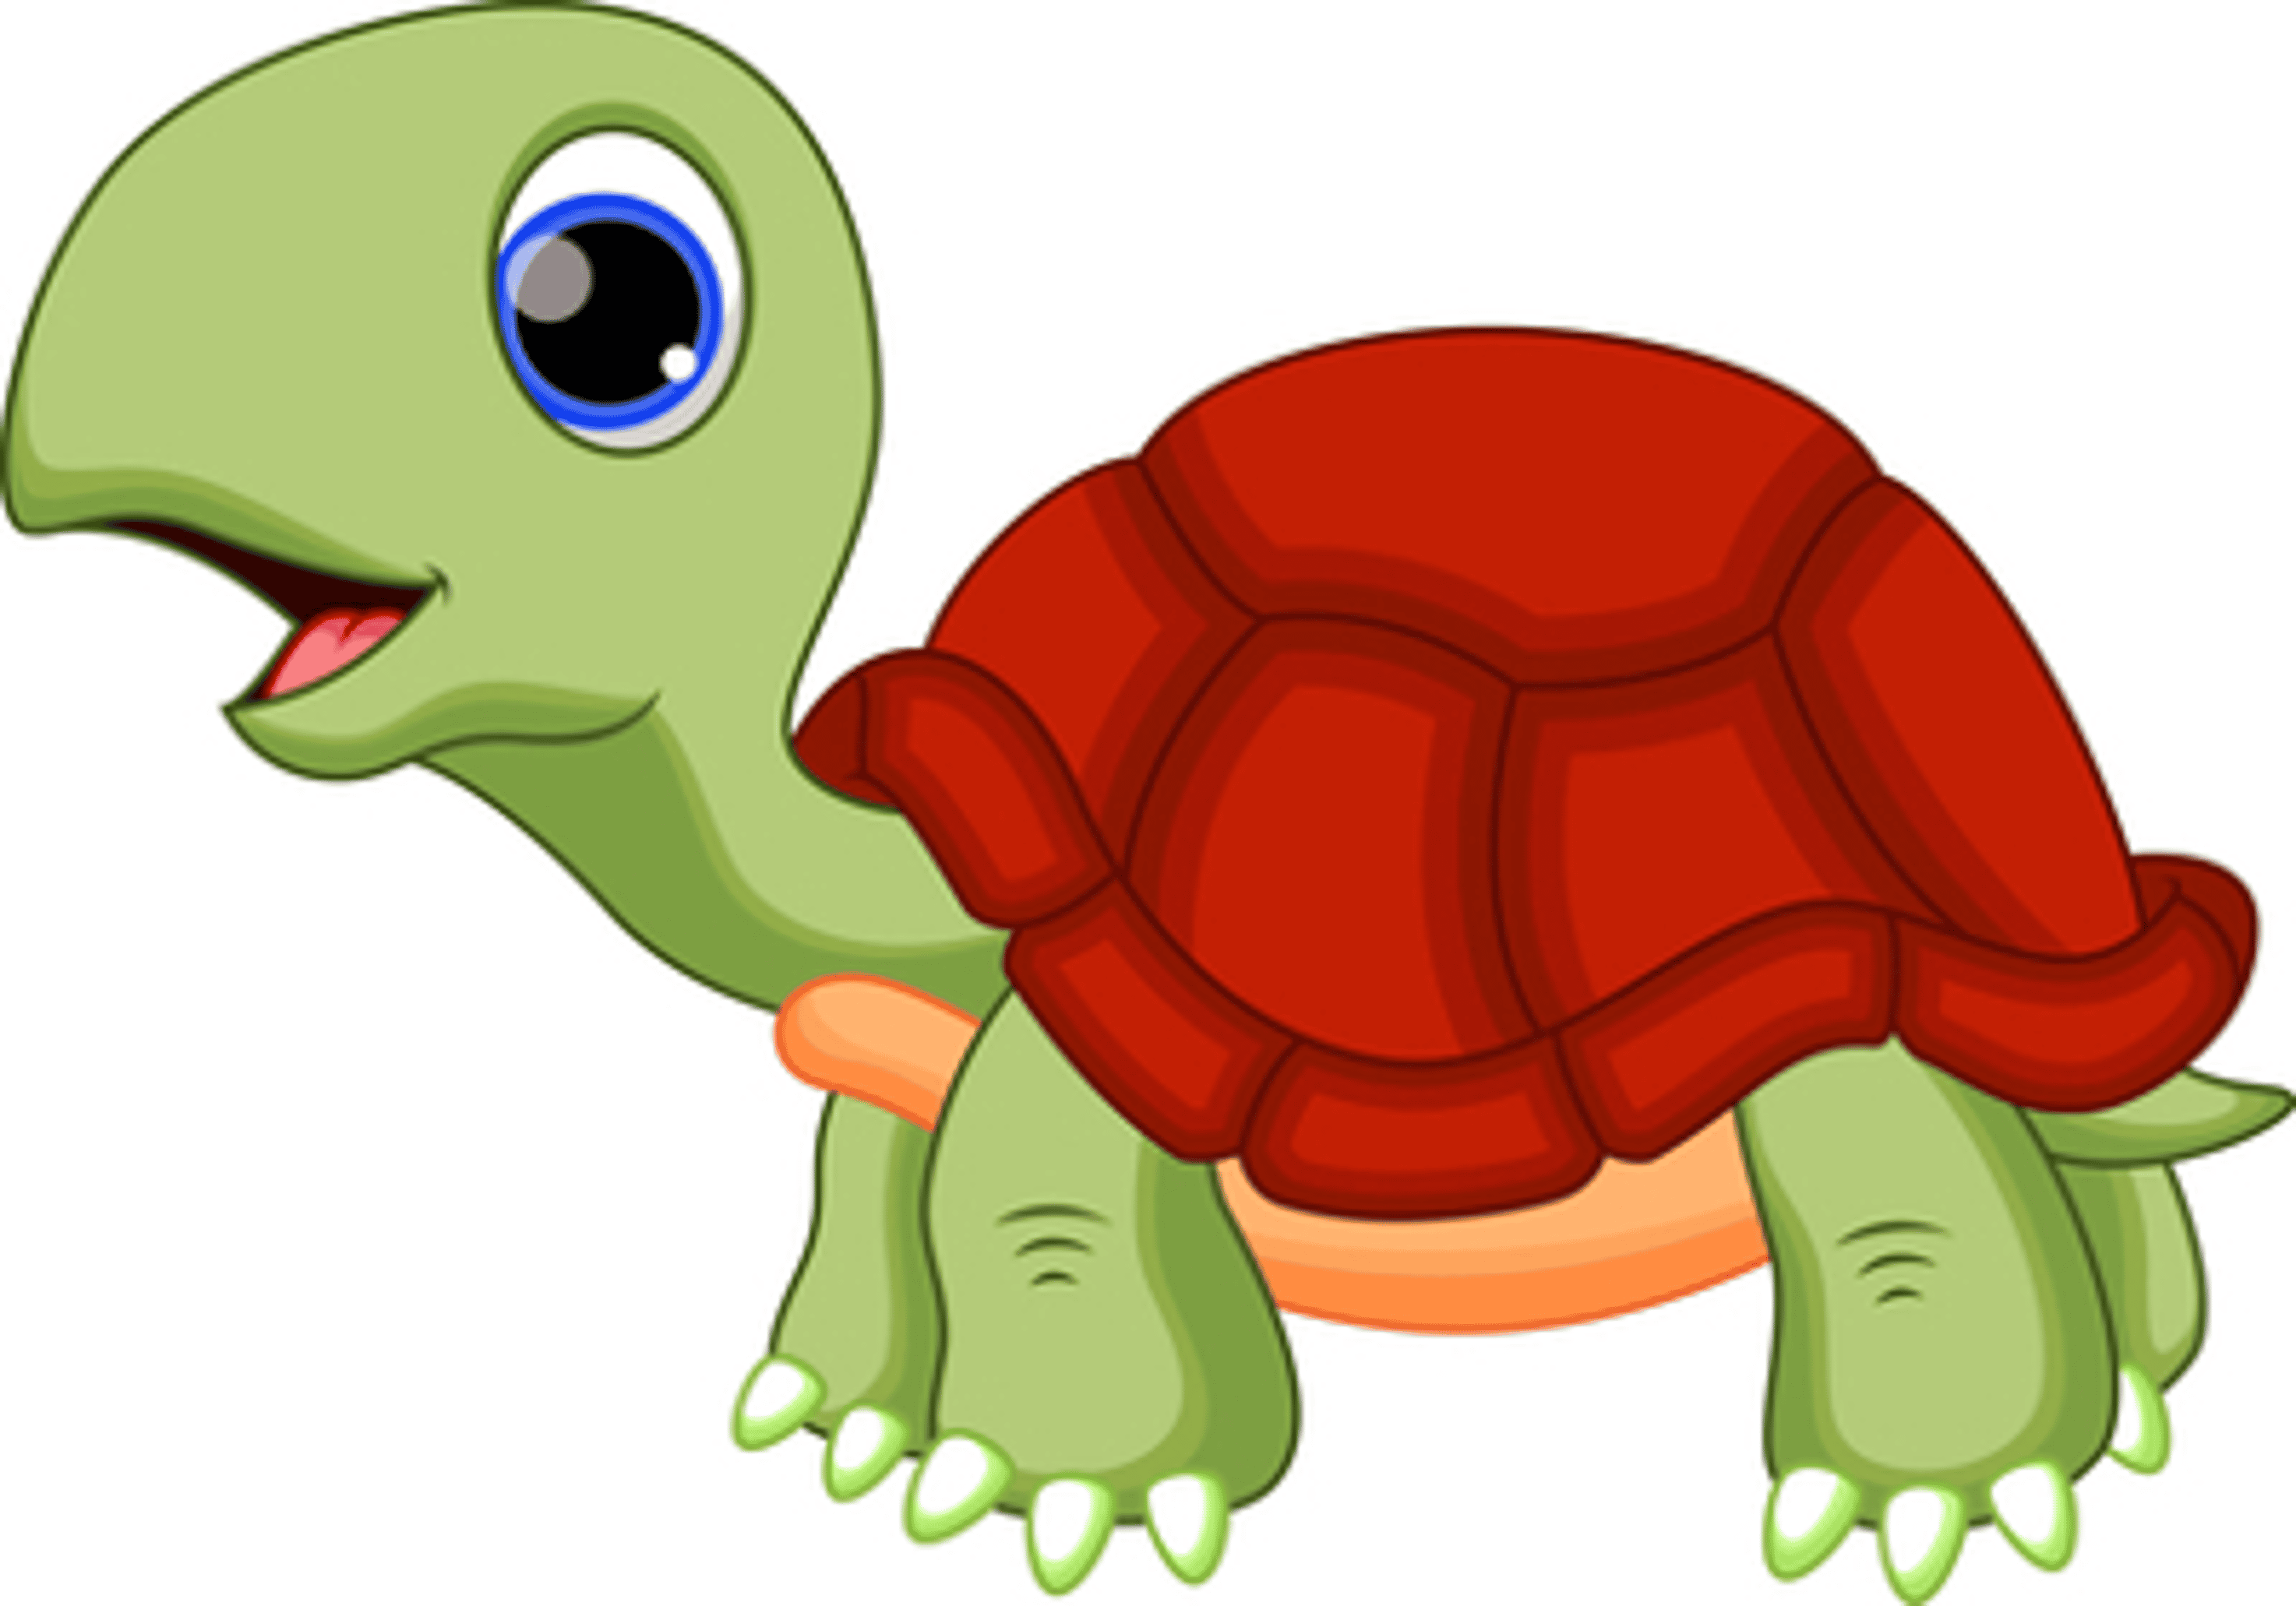
\includegraphics[width=74.25pt,height=56.25pt]{C6M01 - DT - Q5ii.png}};
\draw   (243,76) -- (276,76) -- (276,109) -- (243,109) -- cycle ;
\draw (88,143) node [anchor=north west][inner sep=0.75pt]   [align=left] {150000 green tortoise};
\draw (294,140) node [anchor=north west][inner sep=0.75pt]   [align=left] {130000 red tortoise};
\end{tikzpicture} },
  optionA={$<$},
  optionB={$>$},
  optionC={$=$},
  optionD={None of the above},
  questionTag={C6M01 - DT - Q5}, 
  leftmini={0.5},
  rightmini={0.4},
correctoption={B},
}
% end-of-question

%-----------------------------------------------------------
%                        Question [ 6 ]
%-----------------------------------------------------------
% start-of-question
\mcqfourtabletikz{
   questionnumber={6}, 
  questiontext={Add. },
   tabletikz = {  
      \renewcommand{\arraystretch}{1.5}
      \begin{tabular}{cccccc}
          & 8 & 2 & 5 & 7 & 0  \\
         + & 5 & 8 & 3 & 2 & 0 \\
         \hline
         &&&&&\\
         \hline
      \end{tabular} },
  optionA={1310890},
  optionB={140980},
  optionC={140890},
  optionD={14890},
  questionTag={C6M01 - DT - Q6},
  leftmini={0.5},
  rightmini={0.4},
correctoption={C},
}
% end-of-question

%-----------------------------------------------------------
%                        Question [ 7 ]
%-----------------------------------------------------------
% start-of-question
\mcqfourfour{
  questionnumber={7}, 
  questiontext={Find the remainder of the following.\\
  \qquad   28 $\divisionsymbol$ 9 },
  optionA={1},
  optionB={3},
  optionC={19},
  optionD={37},
  questionTag={C6M01 - DT - Q7}, 
  correctoption={A},
}
% end-of-question

%-----------------------------------------------------------
%                        Question [ 8 ]
%-----------------------------------------------------------
% start-of-question
\mcqfourfour{
  questionnumber={8}, 
  questiontext={1 centimetre is equal to \rule{40pt}{0.5pt} mm.},
  optionA={100 mm},
  optionB={1000 cm},
  optionC={0.1 mm},
  optionD={10 mm},
  questionTag={C6M01 - DT - Q8}, 
  correctoption={D},
}
% end-of-question

%-----------------------------------------------------------
%                        Question [ 9 ]
%-----------------------------------------------------------
% start-of-question
\mcqfourtabletikz{
   questionnumber={9}, 
  questiontext={Match the following.},
  tabletikz = { 
    \renewcommand{\arraystretch}{1.25}
    \begin{tabular}{|p{0.5cm}|p{4cm}|p{0.5cm}|p{0.5cm}|p{3cm}|}
      \cline{1-2}\cline{4-5} 
      \multicolumn{2}{|c|}{\textbf{Column A}} & 
      \multirow{4}[10]{*}{} &   
      \multicolumn{2}{c|}{\textbf{Column B}} \\
      \cline{1-2}\cline{4-5} i & 10 m in cm &   & a & 1000\\
      \cline{1-2}\cline{4-5} ii & 10000 m in km &   & b & 100 \\
      \cline{1-2}\cline{4-5} iii & 1000 mm in cm &   & c & 10 \\
      \cline{1-2}\cline{4-5}
    \end{tabular} },
  optionA={i - c, ii - b, iii - a},
  optionB={i - a, ii - c, iii - b},
  optionC={i - a, ii - b, iii - c},
  optionD={i - b, ii - c, iii - a},
  questionTag={C6M01 - DT - Q9}, 
  correctoption={B},
leftmini={0.7},
rightmini={0.3}
}
% end-of-question

%-----------------------------------------------------------
%                        Question [ 10 ]
%-----------------------------------------------------------
% start-of-question
\mcqfourfour{
  questionnumber={10}, 
  questiontext={Round off the given number to the nearest thousand place.\\
  \qquad  1200},
  optionA={1000},
  optionB={1500},
  optionC={900},
  optionD={2000},
  questionTag={C6M01 - DT - Q10}, 
  correctoption={A},
}
% end-of-question

%-----------------------------------------------------------
%                        Question [ 11 ]
%-----------------------------------------------------------
% start-of-question
\mcqfourfour{
  questionnumber={11}, 
  questiontext={Estimate: 19 $\times$ 78},
  optionA={1480},
  optionB={1500},
  optionC={1600},
  optionD={400},
  questionTag={C6M01 - DT - Q11}, 
  correctoption={C},
}
% end-of-question

%-----------------------------------------------------------
%                        Question [ 12 ]
%-----------------------------------------------------------
% start-of-question
\mcqfourimg{ 
  questionnumber={1}, 
  questiontext={Which flag does not contain a natural number?},
  imgwidth={10cm},
  imgheight={2cm},
  img={C6M03 - DT - Q1.png},
  optionA={Green},
  optionB={Blue},
  optionC={Orange},
  optionD={Red},
  questionTag={C6M03 - DT - Q1}, 
  correctoption={B},
  leftmini={0.5},
  rightmini={0.3},
}
% end-of-question

%-----------------------------------------------------------
%                        Question [ 13 ]
%-----------------------------------------------------------
% start-of-question
\mcqfourfour{
  questionnumber={2}, 
  questiontext={Multiply.\\
  \qquad i.   10 $\times$ 9 = \rule{50pt}{0.5pt}\\
  \qquad ii.  12 $\times$ 19 = \rule{50pt}{0.5pt}},
  optionA={ 90, 120},
  optionB={90, 228},
  optionC={109, 120 },
  optionD={109, 228},
  questionTag={C6M03 - DT - Q2}, 
  correctoption={B},
}
% end-of-question


%-----------------------------------------------------------
%                        Question [ 14 ]
%-----------------------------------------------------------
% start-of-question
\mcqfourtwo{
  questionnumber={3}, 
  questiontext={Which of the following number lines shows 3 × 2?},
  optionA={
\tikzset{every picture/.style={line width=0.75pt}} 
\begin{tikzpicture}[x=0.75pt,y=0.75pt,yscale=-0.75,xscale=0.75]
\draw    (201.35,101.01) -- (540,101.99) (239.37,92.62) -- (239.33,109.62)(277.37,92.73) -- (277.32,109.73)(315.37,92.84) -- (315.32,109.84)(353.37,92.95) -- (353.32,109.95)(391.37,93.06) -- (391.32,110.06)(429.37,93.17) -- (429.32,110.17)(467.37,93.28) -- (467.32,110.28)(505.37,93.39) -- (505.32,110.39) ;
\draw [shift={(543,102)}, rotate = 180.17] [fill={rgb, 255:red, 0; green, 0; blue, 0 }  ][line width=0.08]  [draw opacity=0] (10.72,-5.15) -- (0,0) -- (10.72,5.15) -- (7.12,0) -- cycle    ;
\draw [shift={(199,101)}, rotate = 0.17] [color={rgb, 255:red, 0; green, 0; blue, 0 }  ][line width=0.75]      (0, 0) circle [x radius= 3.35, y radius= 3.35]   ;
\draw  [draw opacity=0][dash pattern={on 4.5pt off 4.5pt}] (238,93.23) .. controls (240.77,69.79) and (266.23,51.69) .. (296.94,52.14) .. controls (327.57,52.59) and (352.42,71.33) .. (354.58,94.76) -- (296.24,97.77) -- cycle ; \draw [dash pattern={on 4.5pt off 4.5pt}] [dash pattern={on 4.5pt off 4.5pt}]  (238,93.23) .. controls (240.77,69.79) and (266.23,51.69) .. (296.94,52.14) .. controls (327.57,52.59) and (352.42,71.33) .. (354.58,94.76) ; \draw [shift={(354.58,94.76)}, rotate = 83.06] [color={rgb, 255:red, 0; green, 0; blue, 0 }  ][fill={rgb, 255:red, 0; green, 0; blue, 0 }  ][dash pattern={on 4.5pt off 4.5pt}][line width=0.75]      (0, 0) circle [x radius= 3.35, y radius= 3.35]   ; 
\draw  [draw opacity=0][dash pattern={on 4.5pt off 4.5pt}] (352.43,95.57) .. controls (353.83,71.25) and (370.71,52.15) .. (391.02,52.44) .. controls (411.3,52.74) and (427.57,72.27) .. (428.28,96.56) -- (390.32,98.53) -- cycle ; \draw [dash pattern={on 4.5pt off 4.5pt}] [dash pattern={on 4.5pt off 4.5pt}]  (352.43,95.57) .. controls (353.83,71.25) and (370.71,52.15) .. (391.02,52.44) .. controls (410.79,52.73) and (426.75,71.3) .. (428.19,94.75) ; \draw [shift={(428.28,96.56)}, rotate = 266.86] [color={rgb, 255:red, 0; green, 0; blue, 0 }  ][dash pattern={on 4.5pt off 4.5pt}][line width=0.75]    (10.93,-4.9) .. controls (6.95,-2.3) and (3.31,-0.67) .. (0,0) .. controls (3.31,0.67) and (6.95,2.3) .. (10.93,4.9)   ; 
\draw (348,116) node [anchor=north west][inner sep=0.75pt]   [align=left] {3};
\draw (272,115) node [anchor=north west][inner sep=0.75pt]   [align=left] {1};
\draw (308,116) node [anchor=north west][inner sep=0.75pt]   [align=left] {2};
\draw (232,115) node [anchor=north west][inner sep=0.75pt]   [align=left] {0};
\draw (386,117) node [anchor=north west][inner sep=0.75pt]   [align=left] {4};
\draw (423,116) node [anchor=north west][inner sep=0.75pt]   [align=left] {5};
\draw (461,115) node [anchor=north west][inner sep=0.75pt]   [align=left] {6};
\draw (499,116) node [anchor=north west][inner sep=0.75pt]   [align=left] {7};
\end{tikzpicture} },
  optionB={
\tikzset{every picture/.style={line width=0.75pt}} 
\begin{tikzpicture}[x=0.75pt,y=0.75pt,yscale=-0.75,xscale=0.75]
\draw    (221.35,121.01) -- (560,121.99) (259.37,112.62) -- (259.33,129.62)(297.37,112.73) -- (297.32,129.73)(335.37,112.84) -- (335.32,129.84)(373.37,112.95) -- (373.32,129.95)(411.37,113.06) -- (411.32,130.06)(449.37,113.17) -- (449.32,130.17)(487.37,113.28) -- (487.32,130.28)(525.37,113.39) -- (525.32,130.39) ;
\draw [shift={(563,122)}, rotate = 180.17] [fill={rgb, 255:red, 0; green, 0; blue, 0 }  ][line width=0.08]  [draw opacity=0] (10.72,-5.15) -- (0,0) -- (10.72,5.15) -- (7.12,0) -- cycle    ;
\draw [shift={(219,121)}, rotate = 0.17] [color={rgb, 255:red, 0; green, 0; blue, 0 }  ][line width=0.75]      (0, 0) circle [x radius= 3.35, y radius= 3.35]   ;
\draw  [draw opacity=0][dash pattern={on 4.5pt off 4.5pt}] (257.87,113.11) .. controls (259.35,89.81) and (276.62,71.55) .. (297.41,71.86) .. controls (318.16,72.16) and (334.84,90.86) .. (335.65,114.13) -- (296.73,116.14) -- cycle ; \draw [dash pattern={on 4.5pt off 4.5pt}] [dash pattern={on 4.5pt off 4.5pt}]  (257.87,113.11) .. controls (259.35,89.81) and (276.62,71.55) .. (297.41,71.86) .. controls (318.16,72.16) and (334.84,90.86) .. (335.65,114.13) ; \draw [shift={(335.65,114.13)}, rotate = 86.41] [color={rgb, 255:red, 0; green, 0; blue, 0 }  ][fill={rgb, 255:red, 0; green, 0; blue, 0 }  ][dash pattern={on 4.5pt off 4.5pt}][line width=0.75]      (0, 0) circle [x radius= 3.35, y radius= 3.35]   ; 
\draw  [draw opacity=0][dash pattern={on 4.5pt off 4.5pt}] (335.91,111.12) .. controls (338.6,88.89) and (363.11,71.74) .. (392.67,72.17) .. controls (422.15,72.61) and (446.07,90.38) .. (448.19,112.59) -- (392,115.5) -- cycle ; \draw [dash pattern={on 4.5pt off 4.5pt}] [dash pattern={on 4.5pt off 4.5pt}]  (335.91,111.12) .. controls (338.6,88.89) and (363.11,71.74) .. (392.67,72.17) .. controls (421.41,72.6) and (444.87,89.5) .. (447.99,110.94) ; \draw [shift={(448.19,112.59)}, rotate = 262.86] [color={rgb, 255:red, 0; green, 0; blue, 0 }  ][dash pattern={on 4.5pt off 4.5pt}][line width=0.75]    (10.93,-4.9) .. controls (6.95,-2.3) and (3.31,-0.67) .. (0,0) .. controls (3.31,0.67) and (6.95,2.3) .. (10.93,4.9)   ; 
\draw (368,136) node [anchor=north west][inner sep=0.75pt]   [align=left] {3};
\draw (292,135) node [anchor=north west][inner sep=0.75pt]   [align=left] {1};
\draw (328,136) node [anchor=north west][inner sep=0.75pt]   [align=left] {2};
\draw (252,135) node [anchor=north west][inner sep=0.75pt]   [align=left] {0};
\draw (406,137) node [anchor=north west][inner sep=0.75pt]   [align=left] {4};
\draw (443,136) node [anchor=north west][inner sep=0.75pt]   [align=left] {5};
\draw (481,135) node [anchor=north west][inner sep=0.75pt]   [align=left] {6};
\draw (519,136) node [anchor=north west][inner sep=0.75pt]   [align=left] {7};
\end{tikzpicture} },
  optionC={
\tikzset{every picture/.style={line width=0.75pt}} 
\begin{tikzpicture}[x=0.75pt,y=0.75pt,yscale=-0.75,xscale=0.75]
\draw    (152.35,124.01) -- (491,124.99) (190.37,115.62) -- (190.33,132.62)(228.37,115.73) -- (228.32,132.73)(266.37,115.84) -- (266.32,132.84)(304.37,115.95) -- (304.32,132.95)(342.37,116.06) -- (342.32,133.06)(380.37,116.17) -- (380.32,133.17)(418.37,116.28) -- (418.32,133.28)(456.37,116.39) -- (456.32,133.39) ;
\draw [shift={(494,125)}, rotate = 180.17] [fill={rgb, 255:red, 0; green, 0; blue, 0 }  ][line width=0.08]  [draw opacity=0] (10.72,-5.15) -- (0,0) -- (10.72,5.15) -- (7.12,0) -- cycle    ;
\draw [shift={(150,124)}, rotate = 0.17] [color={rgb, 255:red, 0; green, 0; blue, 0 }  ][line width=0.75]      (0, 0) circle [x radius= 3.35, y radius= 3.35]   ;
\draw  [draw opacity=0][dash pattern={on 4.5pt off 4.5pt}] (188.87,116.11) .. controls (190.35,92.81) and (207.62,74.55) .. (228.41,74.86) .. controls (249.16,75.16) and (265.84,93.86) .. (266.65,117.13) -- (227.73,119.14) -- cycle ; \draw [dash pattern={on 4.5pt off 4.5pt}] [dash pattern={on 4.5pt off 4.5pt}]  (188.87,116.11) .. controls (190.35,92.81) and (207.62,74.55) .. (228.41,74.86) .. controls (249.16,75.16) and (265.84,93.86) .. (266.65,117.13) ; \draw [shift={(266.65,117.13)}, rotate = 86.41] [color={rgb, 255:red, 0; green, 0; blue, 0 }  ][fill={rgb, 255:red, 0; green, 0; blue, 0 }  ][dash pattern={on 4.5pt off 4.5pt}][line width=0.75]      (0, 0) circle [x radius= 3.35, y radius= 3.35]   ;
\draw  [draw opacity=0][dash pattern={on 4.5pt off 4.5pt}] (266.65,117.13) .. controls (268.14,93.83) and (285.4,75.57) .. (306.19,75.87) .. controls (326.94,76.18) and (343.62,94.87) .. (344.44,118.15) -- (305.51,120.16) -- cycle ; \draw [dash pattern={on 4.5pt off 4.5pt}] [dash pattern={on 4.5pt off 4.5pt}]  (266.65,117.13) .. controls (268.14,93.83) and (285.4,75.57) .. (306.19,75.87) .. controls (326.94,76.18) and (343.62,94.87) .. (344.44,118.15) ; \draw [shift={(344.44,118.15)}, rotate = 86.41] [color={rgb, 255:red, 0; green, 0; blue, 0 }  ][fill={rgb, 255:red, 0; green, 0; blue, 0 }  ][dash pattern={on 4.5pt off 4.5pt}][line width=0.75]      (0, 0) circle [x radius= 3.35, y radius= 3.35]   ;
\draw  [draw opacity=0][dash pattern={on 4.5pt off 4.5pt}] (344.44,118.15) .. controls (345.92,94.85) and (363.19,76.59) .. (383.97,76.89) .. controls (404.72,77.2) and (421.4,95.89) .. (422.22,119.17) -- (383.29,121.18) -- cycle ; \draw [dash pattern={on 4.5pt off 4.5pt}] [dash pattern={on 4.5pt off 4.5pt}]  (344.44,118.15) .. controls (345.92,94.85) and (363.19,76.59) .. (383.97,76.89) .. controls (404.21,77.19) and (420.57,94.97) .. (422.13,117.43) ; \draw [shift={(422.22,119.17)}, rotate = 266.41] [color={rgb, 255:red, 0; green, 0; blue, 0 }  ][dash pattern={on 4.5pt off 4.5pt}][line width=0.75]    (10.93,-4.9) .. controls (6.95,-2.3) and (3.31,-0.67) .. (0,0) .. controls (3.31,0.67) and (6.95,2.3) .. (10.93,4.9)   ; 
\draw (299,139) node [anchor=north west][inner sep=0.75pt]   [align=left] {3};
\draw (223,138) node [anchor=north west][inner sep=0.75pt]   [align=left] {1};
\draw (259,139) node [anchor=north west][inner sep=0.75pt]   [align=left] {2};
\draw (183,138) node [anchor=north west][inner sep=0.75pt]   [align=left] {0};
\draw (337,140) node [anchor=north west][inner sep=0.75pt]   [align=left] {4};
\draw (374,139) node [anchor=north west][inner sep=0.75pt]   [align=left] {5};
\draw (412,138) node [anchor=north west][inner sep=0.75pt]   [align=left] {6};
\draw (450,139) node [anchor=north west][inner sep=0.75pt]   [align=left] {7};
\end{tikzpicture}},
  optionD={
\tikzset{every picture/.style={line width=0.75pt}} 
\begin{tikzpicture}[x=0.75pt,y=0.75pt,yscale=-0.75,xscale=0.75]
\draw    (221.35,121.01) -- (560,121.99) (259.37,112.62) -- (259.33,129.62)(297.37,112.73) -- (297.32,129.73)(335.37,112.84) -- (335.32,129.84)(373.37,112.95) -- (373.32,129.95)(411.37,113.06) -- (411.32,130.06)(449.37,113.17) -- (449.32,130.17)(487.37,113.28) -- (487.32,130.28)(525.37,113.39) -- (525.32,130.39) ;
\draw [shift={(563,122)}, rotate = 180.17] [fill={rgb, 255:red, 0; green, 0; blue, 0 }  ][line width=0.08]  [draw opacity=0] (10.72,-5.15) -- (0,0) -- (10.72,5.15) -- (7.12,0) -- cycle    ;
\draw [shift={(219,121)}, rotate = 0.17] [color={rgb, 255:red, 0; green, 0; blue, 0 }  ][line width=0.75]      (0, 0) circle [x radius= 3.35, y radius= 3.35]   ;
\draw  [draw opacity=0][dash pattern={on 4.5pt off 4.5pt}] (258,113.23) .. controls (260.77,89.79) and (286.23,71.69) .. (316.94,72.14) .. controls (347.57,72.59) and (372.42,91.33) .. (374.58,114.76) -- (316.24,117.77) -- cycle ; \draw [dash pattern={on 4.5pt off 4.5pt}] [dash pattern={on 4.5pt off 4.5pt}]  (258,113.23) .. controls (260.77,89.79) and (286.23,71.69) .. (316.94,72.14) .. controls (347.57,72.59) and (372.42,91.33) .. (374.58,114.76) ; \draw [shift={(374.58,114.76)}, rotate = 83.06] [color={rgb, 255:red, 0; green, 0; blue, 0 }  ][fill={rgb, 255:red, 0; green, 0; blue, 0 }  ][dash pattern={on 4.5pt off 4.5pt}][line width=0.75]      (0, 0) circle [x radius= 3.35, y radius= 3.35]   ; 
\draw  [draw opacity=0][dash pattern={on 4.5pt off 4.5pt}] (335.24,123.08) .. controls (335.89,102.41) and (344.81,85.98) .. (355.44,86.14) .. controls (366.06,86.29) and (374.46,102.94) .. (374.49,123.59) -- (354.85,124.61) -- cycle ; \draw [dash pattern={on 4.5pt off 4.5pt}] [dash pattern={on 4.5pt off 4.5pt}]  (335.34,120.92) .. controls (336.52,101.28) and (345.18,85.99) .. (355.44,86.14) .. controls (366.06,86.29) and (374.46,102.94) .. (374.49,123.59) ;  \draw [shift={(335.24,123.08)}, rotate = 272.74] [color={rgb, 255:red, 0; green, 0; blue, 0 }  ][dash pattern={on 4.5pt off 4.5pt}][line width=0.75]    (10.93,-4.9) .. controls (6.95,-2.3) and (3.31,-0.67) .. (0,0) .. controls (3.31,0.67) and (6.95,2.3) .. (10.93,4.9)   ;
\draw (368,136) node [anchor=north west][inner sep=0.75pt]   [align=left] {3};
\draw (292,135) node [anchor=north west][inner sep=0.75pt]   [align=left] {1};
\draw (328,136) node [anchor=north west][inner sep=0.75pt]   [align=left] {2};
\draw (252,135) node [anchor=north west][inner sep=0.75pt]   [align=left] {0};
\draw (406,137) node [anchor=north west][inner sep=0.75pt]   [align=left] {4};
\draw (443,136) node [anchor=north west][inner sep=0.75pt]   [align=left] {5};
\draw (481,135) node [anchor=north west][inner sep=0.75pt]   [align=left] {6};
\draw (519,136) node [anchor=north west][inner sep=0.75pt]   [align=left] {7};
\end{tikzpicture}
},
  questionTag={C6M03 - DT - Q3}, 
  correctoption={C},
}
% end-of-question

%-----------------------------------------------------------
%                        Question [ 15 ]
%-----------------------------------------------------------
% start-of-question
\mcqfourfour{
  questionnumber={4}, 
  questiontext={Whose statement is correct? \\
  Abi:  $a + b = b + a$ is a closure property.\\
  Anu: $a+(b+c)=(a+b)+c$ is a commutative property.},
  optionA={Abi},
  optionB={Anu},
  optionC={Both are correct},
  optionD={Both are wrong},
  questionTag={C6M03 - DT - Q4}, 
  correctoption={D},
}
% end-of-question

%-----------------------------------------------------------
%                        Question [ 16  ]
%-----------------------------------------------------------
% start-of-question
\mcqfourfour{
  questionnumber={5}, 
  questiontext={Find the next number in the series.\\
  \qquad  5, 15, 11, 21, 17},
  optionA={14},
  optionB={27},
  optionC={7},
  optionD={31},
  questionTag={C6M03 - DT - Q5}, 
  correctoption={B},
}
% end-of-question

%-----------------------------------------------------------
%                        Question [ 17  ]
%-----------------------------------------------------------
% start-of-question
\mcqfourfour{
  questionnumber={6}, 
  questiontext={Find the predecessor of Tuesday.},
  optionA={Tuesday},
  optionB={Wednesday },
  optionC={Monday },
  optionD={Sunday},
  questionTag={C6M03 - DT - Q6}, 
  correctoption={C},
}
% end-of-question

%-----------------------------------------------------------
%                        Question [ 18 ]
%-----------------------------------------------------------
% start-of-question
\mcqfourfour{
  questionnumber={1}, 
  questiontext={Find the set of numbers with one natural number, one whole number and one negative integer.},
  optionA={1, 2, 3},
  optionB={-2, 0, -1},
  optionC={10, 0, -1},
  optionD={-1, 0, 0},
  questionTag={C6M05 - DT - Q1}, 
  correctoption={C},
}
% end-of-question

%-----------------------------------------------------------
%                        Question [ 19 ]
%-----------------------------------------------------------
% start-of-question
\mcqfourfour{
  questionnumber={2}, 
  questiontext={A squirrel jumps 3 points to the left side of the number line. Find the position of the squirrel in the number line.\\
\tikzset{every picture/.style={line width=0.75pt}} 
\hspace{2cm}
\begin{tikzpicture}[x=0.75pt,y=0.75pt,yscale=-1,xscale=1]
\draw (382,82.5) node  {
\includegraphics[width=35pt,height=40pt]{C6M05 - DT - Q2.png}};
\draw    (154,110.01) -- (569,110.99) (192.02,101.6) -- (191.98,118.6)(230.02,101.69) -- (229.98,118.69)(268.02,101.78) -- (267.98,118.78)(306.02,101.87) -- (305.98,118.87)(344.02,101.96) -- (343.98,118.96)(382.02,102.05) -- (381.98,119.05)(420.02,102.14) -- (419.98,119.14)(458.02,102.23) -- (457.98,119.23)(496.02,102.32) -- (495.98,119.32)(534.02,102.41) -- (533.98,119.41) ;
\draw [shift={(572,111)}, rotate = 180.14] [fill={rgb, 255:red, 0; green, 0; blue, 0 }  ][line width=0.08]  [draw opacity=0] (10.72,-5.15) -- (0,0) -- (10.72,5.15) -- (7.12,0) -- cycle    ;
\draw [shift={(151,110)}, rotate = 0.14] [fill={rgb, 255:red, 0; green, 0; blue, 0 }  ][line width=0.08]  [draw opacity=0] (10.72,-5.15) -- (0,0) -- (10.72,5.15) -- (7.12,0) -- cycle    ;
\draw (378,123) node [anchor=north west][inner sep=0.75pt]   [align=left] {0};
\end{tikzpicture}
},
  optionA={+3},
  optionB={-3},
  optionC={-6},
  optionD={+6},
  questionTag={C6M05 - DT - Q2}, 
  correctoption={B},
}
% end-of-question


%-----------------------------------------------------------
%                        Question [ 20 ]
%-----------------------------------------------------------
% start-of-question
\mcqfourfour{
  questionnumber={3}, 
  questiontext={Fill in the blanks with ‘ + ‘ and ‘ - ‘ signs to make the comparison correct. \\
  \hspace{3cm} \rule{30pt}{0.5pt}987  $<$  \rule{30pt}{0.5pt}987},
  optionA={ - 987 $<$ + 987},
  optionB={ - 987 $<$ - 987},
  optionC={ + 987 $<$ + 987},
  optionD={ + 987 $<$ - 987},
  questionTag={C6M05 - DT - Q3}, 
  correctoption={A},
}
% end-of-question

%-----------------------------------------------------------
%                        Question [ 21 ]
%-----------------------------------------------------------
% start-of-question
\mcqfourfour{
  questionnumber={4}, 
  questiontext={Find the greatest integers from the following.},
  optionA={-123},
  optionB={122},
  optionC={-12},
  optionD={0},
  questionTag={C6M05 - DT - Q4}, 
  correctoption={B},
}
% end-of-question

%-----------------------------------------------------------
%                        Question [ 22 ]
%-----------------------------------------------------------
% start-of-question
\mcqfourfour{
  questionnumber={5}, 
  questiontext={Find the correct option.},
  optionA={-3 + (-3) = -6},
  optionB={-3 + 3 = -6},
  optionC={ -3 -3 = 0},
  optionD={3 - 3 = 6 },
  questionTag={C6M05 - DT - Q5}, 
  correctoption={A},
}
% end-of-question

%-----------------------------------------------------------
%                        Question [ 23 ]
%-----------------------------------------------------------
% start-of-question
\mcqfourfour{
  questionnumber={6}, 
  questiontext={Ben participates in a quiz competition. Find the total marks scored by Ben if he got 2 marks for the correct answer and -1 mark for the wrong answer.\\
  \tikzset{every picture/.style={line width=0.75pt}} 
  \hspace{2cm}
\begin{tikzpicture}[x=0.75pt,y=0.75pt,yscale=-0.75,xscale=0.75] 
\draw (321,73) node  {
\includegraphics[width=219.5pt,height=20pt]{C6M05 - DT - Q6.png}};
\draw (111,101) node [anchor=north west][inner sep=0.75pt]   [align=left] {+2 };
\draw (209,101) node [anchor=north west][inner sep=0.75pt]   [align=left] {\mbox{-}1};
\end{tikzpicture}
 },
  optionA={3},
  optionB={-6},
  optionC={1},
  optionD={4},
  questionTag={C6M05 - DT - Q6}, 
  correctoption={D},
}
% end-of-question

%-----------------------------------------------------------
%                        Question [ 24 ]
%-----------------------------------------------------------
% start-of-question
\mcqfourfour{
  questionnumber={7}, 
  questiontext={The addition of two negative numbers always results in \rule{40pt}{0.5pt}.},
  optionA={Zero},
  optionB={Positive number},
  optionC={Negative number},
  optionD={Either a or b },
  questionTag={C6M05 - DT - Q7}, 
  correctoption={C},
}
% end-of-question


%-----------------------------------------------------------
%                        Question [ 25 ]
%-----------------------------------------------------------
% start-of-question
\mcqfourtabletikz{
  questionnumber={1}, 
  questiontext={Find the image with an odd number count.},
  tabletikz = {

\tikzset{every picture/.style={line width=0.75pt}} 
\begin{tikzpicture}[x=0.75pt,y=0.75pt,yscale=-1,xscale=1]
\draw (178.5,110.5) node  {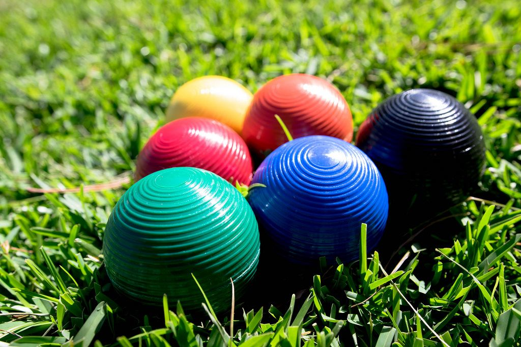
\includegraphics[width=80pt,height=60pt]{C6M04 - DT - Q1i.png}};
\draw (374.5,109.5) node  {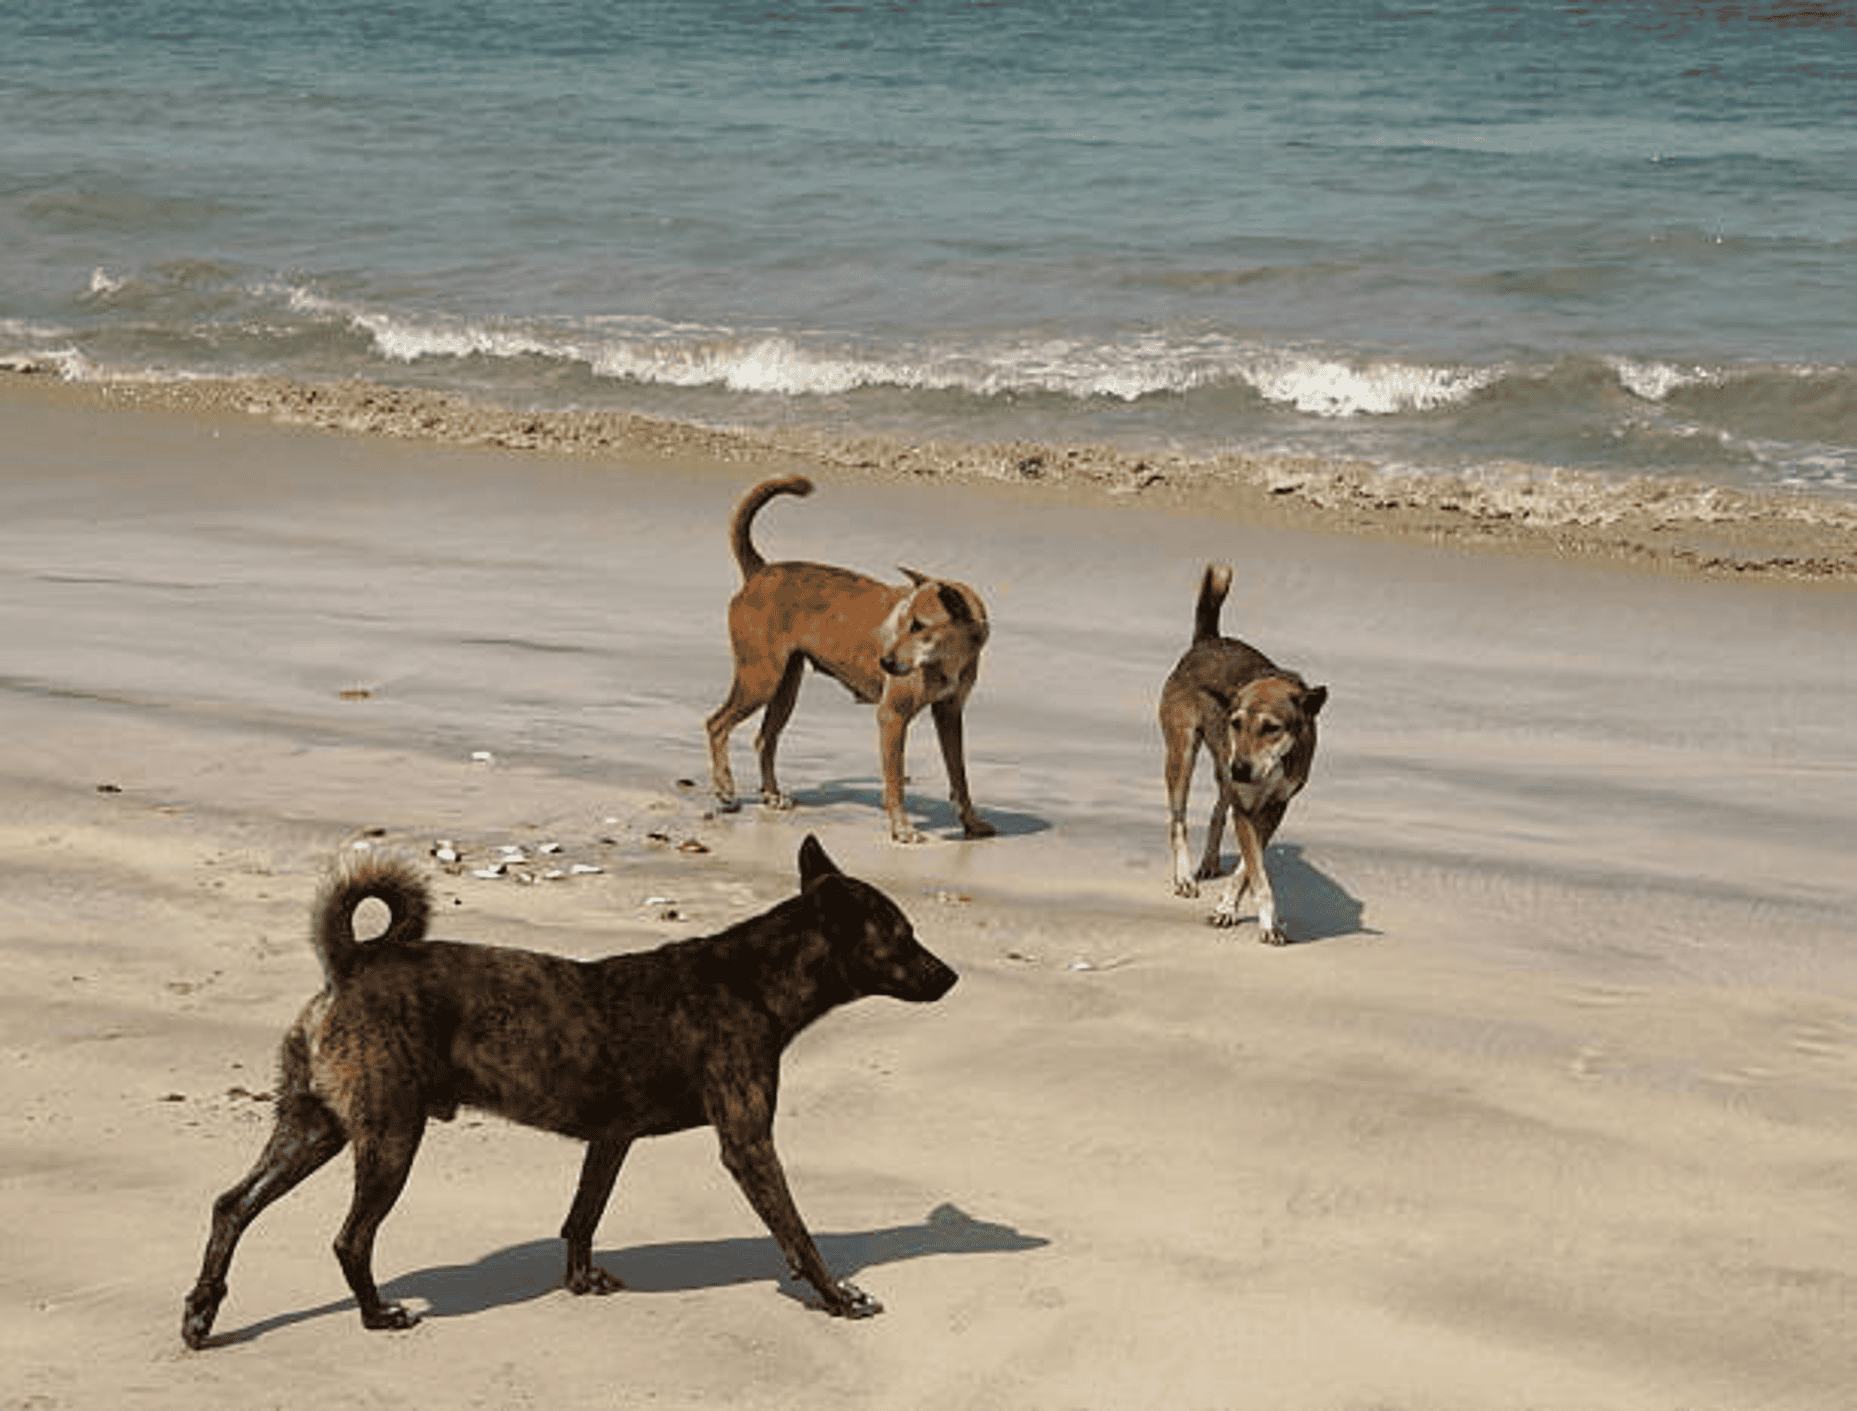
\includegraphics[width=80pt,height=60pt]{C6M04 - DT - Q1ii.png}};
\draw (90,155) node [anchor=north west][inner sep=0.75pt]   [align=left] {Number of balls = \rule{40pt}{0.5pt}};
\draw (295,155) node [anchor=north west][inner sep=0.75pt]   [align=left] {Number of dogs = \rule{40pt}{0.5pt}};
\end{tikzpicture}  
  },
  optionA={Balls},
  optionB={Dogs},
  optionC={Both balls and dogs},
  optionD={None of these},
  questionTag={C6M04 - DT - Q1}, 
  leftmini={0.5},
  rightmini={0.35},
  correctoption={B},
}
% end-of-question

%-----------------------------------------------------------
%                        Question [ 26 ]
%-----------------------------------------------------------
% start-of-question
\mcqfourfour{
  questionnumber={2}, 
  questiontext={Find all the factors of 8.\\
  \smallskip
  \hspace{2cm}
  \colorbox{cyan}{\makebox[1cm][c]{4}} \quad \colorbox{cyan}{\makebox[1cm][c]{1}} \quad
  \colorbox{cyan}{\makebox[1cm][c]{2}} \quad 
  \colorbox{cyan}{\makebox[1cm][c]{6}} \quad 
  \colorbox{cyan}{\makebox[1cm][c]{8}} },
  optionA={1, 2, 8},
  optionB={1, 2, 4, 8},
  optionC={1, 2, 6},
  optionD={4, 6, 8},
  questionTag={C6M04 - DT - Q2}, 
  correctoption={B},
}
% end-of-question

%-----------------------------------------------------------
%                        Question [ 27 ]
%-----------------------------------------------------------
% start-of-question
\mcqfourtabletikz{
  questionnumber={3}, 
  questiontext={Daisy is asked to write the first five multiples of 9.},
  tabletikz = {  1 $\times$ 9 = \rule{40pt}{0.5pt}\\
  2 $\times$ 9 = \rule{40pt}{0.5pt}\\
  3 $\times$ 9 = \rule{40pt}{0.5pt}\\
  4 $\times$ 9 = \rule{40pt}{0.5pt}\\ 
  5 $\times$ 9 = \rule{40pt}{0.5pt}},
  optionA={9, 11, 12, 13, 14},
  optionB={9, 18, 36, 45, 54},
  optionC={9, 18, 27, 36, 45},
  optionD={19, 29, 39, 49, 59},
  questionTag={C6M04 – DT – Q3}, 
  correctoption={C},
  leftmini={0.5},
   rightmini={0.5}
}
% end-of-question

%-----------------------------------------------------------
%                        Question [ 28 ]
%-----------------------------------------------------------
% start-of-question
\mcqfourtabletikz{
  questionnumber={4}, 
  questiontext={Match the numbers with types of numbers.},
  tabletikz = {
    \renewcommand{\arraystretch}{1.25}
    \begin{tabular}{|p{0.5cm}|p{1.6cm}|p{0.2cm}|p{0.5cm}|p{5.3cm}|}
      \cline{1-2}\cline{4-5} 
      \multicolumn{2}{|c|}{\textbf{Numbers}} & 
      \multirow{4}[10]{*}{} &   
      \multicolumn{2}{c|}{\textbf{Type of Numbers }} \\
      \cline{1-2}\cline{4-5} i & 1 &   & a & Neither prime nor composite \\
      \cline{1-2}\cline{4-5} ii & 10 &   & b & Composite numbers  \\
      \cline{1-2}\cline{4-5} iii & 5 &   & c & Prime numbers \\
      \cline{1-2}\cline{4-5}
    \end{tabular} },
  optionA={i - c, ii - b, iii - a},
  optionB={i - a, ii - c, iii - b},
  optionC={i - a, ii - b, iii - c},
  optionD={i - b, ii - a, iii - c},
  questionTag={C6M04 – DT – Q4}, 
  correctoption={C},
  leftmini={0.5},
    rightmini={0.35}
}
% end-of-question

%-----------------------------------------------------------
%                        Question [ 29 ]
%-----------------------------------------------------------
% start-of-question
\mcqfourfour{
  questionnumber={5}, 
  questiontext={Find the unit digit of the number 7910.},
  optionA={0},
  optionB={4},
  optionC={7},
  optionD={1},
  questionTag={C6M04 - DT - Q5}, 
  correctoption={A},
}
% end-of-question

%-----------------------------------------------------------
%                        Question [ 30 ]
%-----------------------------------------------------------
% start-of-question
\mcqfourimg{
  questionnumber={6}, 
  questiontext={The given amount is divisible by \rule{40pt}{0.5pt}.},
  imgwidth={6cm},
  imgheight={2.5cm},
  img={C6M04 - DT - Q6.png},
  optionA={5},
  optionB={3},
  optionC={4},
  optionD={6},
  questionTag={C6M04 - DT - Q6}, 
  leftmini={0.4},
  rightmini={0.4},
  correctoption={A},
}
% end-of-question

%-----------------------------------------------------------
%                        Question [ 31 ]
%-----------------------------------------------------------
% start-of-question
\mcqfourtabletikz{
  questionnumber={7}, 
  questiontext={Find the prime factors of 18.},
  tabletikz = { 
       \renewcommand{\arraystretch}{1.3}
      \begin{tabular}{p{1cm}|p{2cm}}
          \RaggedLeft{2} & 18 \\
          \cline{2-2}
          & \\
          \cline{2-2}
          & \\
          \cline{2-2}
          & 1 \\
          \cline{2-2}          
      \end{tabular}
  },
  optionA={ 2 $\times$ 6 $\times$ 1},
  optionB={2 $\times$ 2 $\times$ 3},
  optionC={2 $\times$ 3 $\times$ 3},
  optionD={6 $\times$ 1 $\times$ 3},
  questionTag={C6M04 - DT - Q7},
  leftmini={0.5},
  rightmini={0.4},
  correctoption={C},
}
% end-of-question

%-----------------------------------------------------------
%                        Question [ 32 ]
%-----------------------------------------------------------
% start-of-question
\mcqfourtabletikz{
  questionnumber={8}, 
  questiontext={Find the number in the circle by completing the given LCM. },
  tabletikz = { 
   \renewcommand{\arraystretch}{1.25}
      \begin{tabular}{p{1cm}|p{0.5cm}p{1cm}}
          \RaggedLeft{2} & 4, & 6 \\
          \cline{2-3}
          \RaggedLeft{2} & 2,& \rule{20pt}{0.5pt}\\
          \cline{2-3}
          \RaggedLeft{{\large{\textcircled{\rule{10pt}{0.5pt}}}}} & \rule{20pt}{0.5pt}, & 3 \\
          \cline{2-3}
          & 1,& 1 \\
          \cline{2-3}          
      \end{tabular}
       },
  optionA={1},
  optionB={2},
  optionC={0},
  optionD={3},
  questionTag={C6M04 - DT - Q8}, 
  leftmini={0.5},
  rightmini={0.4},
  correctoption={D},
}
% end-of-question

%-----------------------------------------------------------
%                        Question [ 33 ]
%-----------------------------------------------------------
% start-of-question
\mcqfourfour{
  questionnumber={9}, 
  questiontext={Find the highest common factor of 9 and 18.\\
   \quad The factors of 9 are 1, 3 and 9.\\
   \quad The factors of 18 are 1, 2, 3, 6, 9 and 18. },
  optionA={1, 3, 9},
  optionB={1, 3},
  optionC={18},
  optionD={9},
  questionTag={C6M04 - DT - Q9}, 
  correctoption={D},
}
% end-of-question

%-----------------------------------------------------------
%                        Question [ 34 ]
%-----------------------------------------------------------
% start-of-question
\mcqfourfour{
  questionnumber={1}, 
  questiontext={Count the number of points.\\
  \medskip
  \tikzset{every picture/.style={line width=0.75pt}} 
\hspace{2cm}
\begin{tikzpicture}[x=0.75pt,y=0.75pt,yscale=-1,xscale=1]
\draw    (102,111.97) -- (405,107.03) ;
\draw [shift={(407,107)}, rotate = 179.07] [color={rgb, 255:red, 0; green, 0; blue, 0 }  ][line width=0.75]    (10.93,-4.9) .. controls (6.95,-2.3) and (3.31,-0.67) .. (0,0) .. controls (3.31,0.67) and (6.95,2.3) .. (10.93,4.9)   ;
\draw [shift={(100,112)}, rotate = 359.07] [color={rgb, 255:red, 0; green, 0; blue, 0 }  ][line width=0.75]    (10.93,-4.9) .. controls (6.95,-2.3) and (3.31,-0.67) .. (0,0) .. controls (3.31,0.67) and (6.95,2.3) .. (10.93,4.9)   ;
\draw  [fill={rgb, 255:red, 74; green, 74; blue, 74 }  ,fill opacity=1 ] (147,112.5) .. controls (147,110.57) and (148.57,109) .. (150.5,109) .. controls (152.43,109) and (154,110.57) .. (154,112.5) .. controls (154,114.43) and (152.43,116) .. (150.5,116) .. controls (148.57,116) and (147,114.43) .. (147,112.5) -- cycle ;
\draw  [fill={rgb, 255:red, 74; green, 74; blue, 74 }  ,fill opacity=1 ] (196,110.5) .. controls (196,108.57) and (197.57,107) .. (199.5,107) .. controls (201.43,107) and (203,108.57) .. (203,110.5) .. controls (203,112.43) and (201.43,114) .. (199.5,114) .. controls (197.57,114) and (196,112.43) .. (196,110.5) -- cycle ;
\draw  [fill={rgb, 255:red, 74; green, 74; blue, 74 }  ,fill opacity=1 ] (255,109.5) .. controls (255,107.57) and (256.57,106) .. (258.5,106) .. controls (260.43,106) and (262,107.57) .. (262,109.5) .. controls (262,111.43) and (260.43,113) .. (258.5,113) .. controls (256.57,113) and (255,111.43) .. (255,109.5) -- cycle ;
\draw  [fill={rgb, 255:red, 74; green, 74; blue, 74 }  ,fill opacity=1 ] (293,109.5) .. controls (293,107.57) and (294.57,106) .. (296.5,106) .. controls (298.43,106) and (300,107.57) .. (300,109.5) .. controls (300,111.43) and (298.43,113) .. (296.5,113) .. controls (294.57,113) and (293,111.43) .. (293,109.5) -- cycle ;
\draw  [fill={rgb, 255:red, 74; green, 74; blue, 74 }  ,fill opacity=1 ] (347,108.5) .. controls (347,106.57) and (348.57,105) .. (350.5,105) .. controls (352.43,105) and (354,106.57) .. (354,108.5) .. controls (354,110.43) and (352.43,112) .. (350.5,112) .. controls (348.57,112) and (347,110.43) .. (347,108.5) -- cycle ;
\end{tikzpicture}
},
  optionA={Four},
  optionB={Five},
  optionC={One},
  optionD={Zero},
  questionTag={C6M11 – DT – Q1}, 
  correctoption={B},
}
% end-of-question

%-----------------------------------------------------------
%                        Question [ 35 ]
%-----------------------------------------------------------
% start-of-question
\mcqfourtabletikz{
  questionnumber={2}, 
  questiontext={Match the following.},
  tabletikz = { 
    \renewcommand{\arraystretch}{1.25}
    \begin{tabular}{|p{0.5cm}|p{2.5cm}|p{0.3cm}|p{0.5cm}|p{3.5cm}|}
      \cline{1-2}\cline{4-5} 
      \multicolumn{2}{|c|}{\textbf{Symbols}} & 
      \multirow{4}[10]{*}{} &   
      \multicolumn{2}{c|}{\textbf{Name}} \\
      \cline{1-2}\cline{4-5} i & 

\tikzset{every picture/.style={line width=0.75pt}} 
\begin{tikzpicture}[x=0.75pt,y=0.75pt,yscale=-1,xscale=1]
\draw    (100,120) -- (172,120) ;
\draw [shift={(174,120)}, rotate = 180] [color={rgb, 255:red, 0; green, 0; blue, 0 }  ][line width=0.75]    (10.93,-4.9) .. controls (6.95,-2.3) and (3.31,-0.67) .. (0,0) .. controls (3.31,0.67) and (6.95,2.3) .. (10.93,4.9)   ;
\draw [shift={(100,120)}, rotate = 0] [color={rgb, 255:red, 0; green, 0; blue, 0 }  ][fill={rgb, 255:red, 0; green, 0; blue, 0 }  ][line width=0.75]      (0, 0) circle [x radius= 3.35, y radius= 3.35]   ;
\end{tikzpicture}
 &   & a & Line segment\\
      \cline{1-2}\cline{4-5} ii &  

\tikzset{every picture/.style={line width=0.75pt}} 
\begin{tikzpicture}[x=0.75pt,y=0.75pt,yscale=-1,xscale=1]
\draw    (102,120) -- (172,120) ;
\draw [shift={(174,120)}, rotate = 180] [color={rgb, 255:red, 0; green, 0; blue, 0 }  ][line width=0.75]    (10.93,-4.9) .. controls (6.95,-2.3) and (3.31,-0.67) .. (0,0) .. controls (3.31,0.67) and (6.95,2.3) .. (10.93,4.9)   ;
\draw [shift={(100,120)}, rotate = 0] [color={rgb, 255:red, 0; green, 0; blue, 0 }  ][line width=0.75]    (10.93,-4.9) .. controls (6.95,-2.3) and (3.31,-0.67) .. (0,0) .. controls (3.31,0.67) and (6.95,2.3) .. (10.93,4.9)   ;
\end{tikzpicture}
&   & b & Ray\\
      \cline{1-2}\cline{4-5} iii & 

\tikzset{every picture/.style={line width=0.75pt}} 
\begin{tikzpicture}[x=0.75pt,y=0.75pt,yscale=-1,xscale=1]
\draw    (100,120) -- (174,120) ;
\draw [shift={(174,120)}, rotate = 0] [color={rgb, 255:red, 0; green, 0; blue, 0 }  ][fill={rgb, 255:red, 0; green, 0; blue, 0 }  ][line width=0.75]      (0, 0) circle [x radius= 3.35, y radius= 3.35]   ;
\draw [shift={(100,120)}, rotate = 0] [color={rgb, 255:red, 0; green, 0; blue, 0 }  ][fill={rgb, 255:red, 0; green, 0; blue, 0 }  ][line width=0.75]      (0, 0) circle [x radius= 3.35, y radius= 3.35]   ;
\end{tikzpicture}
&   & c & Line \\
      \cline{1-2}\cline{4-5}
    \end{tabular} },
  optionA={i - b, ii - c, iii - a},
  optionB={i - a, ii - b, iii - c},
  optionC={i - c, ii - b, iii - a},
  optionD={i - a, ii - c, iii - b},
  questionTag={C6M11 – DT – Q2}, 
  correctoption={A},
  leftmini={0.5},
    rightmini={0.35}
}
% end-of-question

%-----------------------------------------------------------
%                        Question [ 36 ]
%-----------------------------------------------------------
% start-of-question
\mcqfourimg{
  questionnumber={3}, 
  questiontext={The given lines are \rule{80pt}{0.5pt}.},
  imgwidth={2.5cm},
  imgheight={2.5cm},
  img={C6M11 - DT - Q3.png},
  optionA={Perpendicular lines},
  optionB={Intersecting lines},
  optionC={Parallel lines},
  optionD={None of these},
  questionTag={C6M11 - DT - Q3}, 
  correctoption={C},
  leftmini={0.3},
  rightmini={0.6}
}
% end-of-question
%-----------------------------------------------------------
%                        Question [ 33 ]
%-----------------------------------------------------------
% start-of-question
\mcqfourfour{
  questionnumber={4}, 
  questiontext={Which teddy bear shows an incorrect measurement of angles?},
  optionA={ 
\includegraphics[height= 2cm, width=2.8cm]{C6M11 - DT - Q4i.png}  },
  optionB={
\includegraphics[height= 2cm, width=2.8cm]{C6M11 - DT - Q4ii.png}  },
  optionC={
\includegraphics[height= 2cm, width=2.8cm]{C6M11 - DT - Q4iii.png} },
  optionD={ All the above},
  questionTag={C6M11 - DT - Q4}, 
  correctoption={D},
}
% end-of-question

%-----------------------------------------------------------
%                        Question [ 37 ]
%-----------------------------------------------------------
% start-of-question
\mcqfourtabletikz{
  questionnumber={5}, 
  questiontext={The adjacent angles in the given figure are $\angle$XOY and \rule{50pt}{0.5pt}.},
  tabletikz = {
  \tikzset{every picture/.style={line width=0.75pt}} 
\begin{tikzpicture}[x=0.75pt,y=0.75pt,yscale=-0.8,xscale=0.8]
\draw    (147,131) -- (263.4,44.2) ;
\draw [shift={(265,43)}, rotate = 143.29] [color={rgb, 255:red, 0; green, 0; blue, 0 }  ][line width=0.75]    (10.93,-4.9) .. controls (6.95,-2.3) and (3.31,-0.67) .. (0,0) .. controls (3.31,0.67) and (6.95,2.3) .. (10.93,4.9)   ;
\draw    (147,130) -- (290.04,99.42) ;
\draw [shift={(292,99)}, rotate = 167.93] [color={rgb, 255:red, 0; green, 0; blue, 0 }  ][line width=0.75]    (10.93,-4.9) .. controls (6.95,-2.3) and (3.31,-0.67) .. (0,0) .. controls (3.31,0.67) and (6.95,2.3) .. (10.93,4.9)   ; 
\draw    (147,131) -- (302,131) ;
\draw [shift={(304,131)}, rotate = 180] [color={rgb, 255:red, 0; green, 0; blue, 0 }  ][line width=0.75]    (10.93,-4.9) .. controls (6.95,-2.3) and (3.31,-0.67) .. (0,0) .. controls (3.31,0.67) and (6.95,2.3) .. (10.93,4.9)   ;
\draw (122,132) node [anchor=north west][inner sep=0.75pt]   [align=left] {O};
\draw (271,24) node [anchor=north west][inner sep=0.75pt]   [align=left] {X};
\draw (295,83) node [anchor=north west][inner sep=0.75pt]   [align=left] {Y};
\draw (309,125) node [anchor=north west][inner sep=0.75pt]   [align=left] {Z};
\end{tikzpicture}

  },
  optionA={$\angle$XOZ},
  optionB={$\angle$YOX},
  optionC={$\angle$YOZ},
  optionD={$\angle$XYZ},
  questionTag={C6M11 - DT - Q5}, 
  correctoption={C},
  leftmini={0.5},
    rightmini={0.5}
}
% end-of-question

%-----------------------------------------------------------
%                        Question [ 38 ]
%-----------------------------------------------------------
% start-of-question
\mcqfourfour{
  questionnumber={6}, 
  questiontext={Find the linear pair of angles.},
  optionA={$180^\circ$, $180^\circ$},
  optionB={$180^\circ$, $90^\circ$},
  optionC={$90^\circ$ , $180^\circ$},
  optionD={$90^\circ$, $90^\circ$},
  questionTag={C6M11 - DT - Q6}, 
  correctoption={D}
}
% end-of-question

%-----------------------------------------------------------
%                        Question [ 36 ]
%-----------------------------------------------------------
% start-of-question
\mcqfourfour{
  questionnumber={7}, 
  questiontext={Find the figure with an open curve.},
  optionA={
\tikzset{every picture/.style={line width=0.75pt}} 
\begin{tikzpicture}[x=0.75pt,y=0.75pt,yscale=-0.75,xscale=0.75] 
\draw   (100,121) -- (198,121) -- (180.06,134) -- (112,134) -- (112,183.31) -- (100,192) -- cycle ;
\end{tikzpicture} },
  optionB={
\tikzset{every picture/.style={line width=0.75pt}} 
\begin{tikzpicture}[x=0.75pt,y=0.75pt,yscale=-0.75,xscale=0.75]
\draw   (270,45.5) .. controls (270,32.52) and (280.52,22) .. (293.5,22) .. controls (306.48,22) and (317,32.52) .. (317,45.5) .. controls (317,58.48) and (306.48,69) .. (293.5,69) .. controls (280.52,69) and (270,58.48) .. (270,45.5)(258,45.5) .. controls (258,25.89) and (273.89,10) .. (293.5,10) .. controls (313.11,10) and (329,25.89) .. (329,45.5) .. controls (329,65.11) and (313.11,81) .. (293.5,81) .. controls (273.89,81) and (258,65.11) .. (258,45.5) ;
\end{tikzpicture} },
  optionC={
 \tikzset{every picture/.style={line width=0.75pt}} 
\begin{tikzpicture}[x=0.75pt,y=0.75pt,yscale=-0.75,xscale=0.75]
\draw   (373.19,149.4) .. controls (376.26,155.12) and (378,161.61) .. (378,168.5) .. controls (378,191.42) and (358.75,210) .. (335,210) .. controls (311.25,210) and (292,191.42) .. (292,168.5) .. controls (292,145.58) and (311.25,127) .. (335,127) -- (335,168.5) -- cycle ;
\end{tikzpicture} },
  optionD={
\tikzset{every picture/.style={line width=0.75pt}} 
\begin{tikzpicture}[x=0.75pt,y=0.75pt,yscale=-0.75,xscale=0.75] 
\draw  [draw opacity=0] (542.03,145.92) .. controls (547.81,141.58) and (555.09,139) .. (563,139) .. controls (581.78,139) and (597,153.55) .. (597,171.5) .. controls (597,189.45) and (581.78,204) .. (563,204) .. controls (546.07,204) and (532.03,192.17) .. (529.43,176.69) -- (563,171.5) -- cycle ; \draw   (542.03,145.92) .. controls (547.81,141.58) and (555.09,139) .. (563,139) .. controls (581.78,139) and (597,153.55) .. (597,171.5) .. controls (597,189.45) and (581.78,204) .. (563,204) .. controls (546.07,204) and (532.03,192.17) .. (529.43,176.69) ;  
\end{tikzpicture} },
  questionTag={C6M11 – DT – Q7}, 
  correctoption={D},
}
% end-of-question

%-----------------------------------------------------------
%                        Question [ 39 ]
%-----------------------------------------------------------
% start-of-question
\mcqfourimg{
  questionnumber={1}, 
  questiontext={Name this polygon.},
  imgwidth={5cm},
  imgheight={3cm},
  img={C6M12 - DT - Q1.png},
  optionA={Square},
  optionB={Heptagon},
  optionC={Octagon},
  optionD={Pentagon},
  questionTag={C6M12 - DT - Q1}, 
  correctoption={C},
  leftmini={0.45},
  rightmini={0.45},
}
% end-of-question

%-----------------------------------------------------------
%                        Question [ 40 ]
%-----------------------------------------------------------
% start-of-question
\mcqfourtwo{
  questionnumber={2}, 
  questiontext={Find the odd one out. },
  optionA={Scalene triangle - three unequal sides},
  optionB={Isosceles triangle - two equal sides},
  optionC={Equilateral triangle - three equal sides},
  optionD={Right angled triangle – all sides equal },
  questionTag={C6M12 - DT - Q2}, 
  correctoption={D},
}
% end-of-question

%-----------------------------------------------------------
%                        Question [ 41 ]
%-----------------------------------------------------------
% start-of-question

\mcqfourimg{
  questionnumber={3}, 
  questiontext={Match the following.},
  imgwidth={8cm},
  imgheight={4cm},
  img={C6M12 - DT - Q3.png},
   optionA={i - c, ii - d, iii - a, iv - b},
  optionB={i - c, ii - b, iii - a, iv - d},
  optionC={i - c, ii - d, iii - b, iv - a},
  optionD={i - b, ii - a, iii - c, iv - d},
  questionTag={C6M12 – DT – Q3}, 
  leftmini={0.5},
  rightmini={0.5}, 
  correctoption={C},
}
% end-of-question

%-----------------------------------------------------------
%                        Question [ 42 ]
%-----------------------------------------------------------
% start-of-question
\mcqfourtabletikz{
  questionnumber={4}, 
  questiontext={What does the line in the given figure represent?},
  tabletikz = {\tikzset{every picture/.style={line width=0.75pt}}
\hspace{3cm}
\begin{tikzpicture}[x=0.75pt,y=0.75pt,yscale=-0.75,xscale=0.75]
\draw    (86.5,105) -- (199.5,105) ;
\draw [shift={(202.5,105)}, rotate = 180] [fill={rgb, 255:red, 0; green, 0; blue, 0 }  ][line width=0.08]  [draw opacity=0] (6.25,-3) -- (0,0) -- (6.25,3) -- cycle    ;
\draw [shift={(83.5,105)}, rotate = 0] [fill={rgb, 255:red, 0; green, 0; blue, 0 }  ][line width=0.08]  [draw opacity=0] (6.25,-3) -- (0,0) -- (6.25,3) -- cycle    ; 
\draw   (83.5,105) .. controls (83.5,72.14) and (110.14,45.5) .. (143,45.5) .. controls (175.86,45.5) and (202.5,72.14) .. (202.5,105) .. controls (202.5,137.86) and (175.86,164.5) .. (143,164.5) .. controls (110.14,164.5) and (83.5,137.86) .. (83.5,105) -- cycle ;
\draw (135,85) node [anchor=north west][inner sep=0.75pt]   [align=left] {?};
\end{tikzpicture}},
  optionA={Radius},
  optionB={Vertices},
  optionC={Diameter},
  optionD={Circumference},
  questionTag={C6M12 - DT - Q4}, 
  correctoption={C},
  leftmini={0.5},
    rightmini={0.5}
}
% end-of-question

%-----------------------------------------------------------
%                        Question [ 43 ]
%-----------------------------------------------------------

% start-of-question
\mcqfourtwo{
  questionnumber={1}, 
  questiontext={3D shapes have \rule{80pt}{0.5pt}.},
  optionA={Only length},
  optionB={Length and breadth},
  optionC={Only height},
  optionD={ Length, breadth and height},
  questionTag={C6M13 – DT – Q1}, 
  correctoption={D},
}
% end-of-question


%-----------------------------------------------------------
%                        Question [ 44 ]
%-----------------------------------------------------------
% start-of-question
\mcqfourimg{
  questionnumber={2}, 
  questiontext={Identify the colour of the vertices.},
  imgwidth={5cm},
  imgheight={3cm},
  img={C6M13 - DT - Q2.png},
  optionA={Pink },
  optionB={Blue},
  optionC={Green },
  optionD={Grey},
  questionTag={C6M13 - DT - Q2}, 
  correctoption={B},
  leftmini={0.5},
  rightmini={0.5}
}
% end-of-question

%-----------------------------------------------------------
%                        Question [ 45 ]
%-----------------------------------------------------------
% start-of-question
\mcqfourimg{
  questionnumber={1}, 
  questiontext={Represent the given number of ice creams in tallymarks.},
  imgwidth={8cm},
  imgheight={1.5cm},
  img={C6M17 - DT - Q1.png},
  optionA={
  \tikzset{every picture/.style={line width=0.75pt}} 
\begin{tikzpicture}[x=0.75pt,y=0.75pt,yscale=-0.75,xscale=0.75] 
\draw    (191,100) -- (191,117.8) ; 
\draw    (201.4,100) -- (201.4,117.8) ;
\draw    (195.8,100) -- (195.8,117.8) ; 
\draw    (204,103) -- (189,115.8) ;
\draw    (207.8,100) -- (207.8,117.8) ;
\end{tikzpicture}},
  optionB={
  \tikzset{every picture/.style={line width=0.75pt}} 
\begin{tikzpicture}[x=0.75pt,y=0.75pt,yscale=-0.75,xscale=0.75] 
\draw    (258,101.4) -- (258,119.2) ; 
\draw    (268.4,101.4) -- (268.4,119.2) ;
\draw    (262.8,101.4) -- (262.8,119.2) ;
\draw    (273.2,101.2) -- (273.2,119) ;
\draw    (278.8,101.4) -- (278.8,119.2) ;
\draw    (283.6,101.4) -- (283.6,119.2) ;
\end{tikzpicture}  },
  optionC={ 
\tikzset{every picture/.style={line width=0.75pt}} 
\begin{tikzpicture}[x=0.75pt,y=0.75pt,yscale=-0.75,xscale=0.75]
\draw    (358,82.2) -- (358,100) ;
\draw    (362.8,82.2) -- (362.8,100) ;
\draw    (365.8,83.2) -- (355,97) ;
\draw    (373.2,81.4) -- (373.2,99.2) ; 
\draw    (378,81.4) -- (378,99.2) ; 
\draw    (381,82.4) -- (370.2,96.2) ;
\draw    (389.2,81.4) -- (389.2,99.2) ;
\draw    (394,81.4) -- (394,99.2) ; 
\draw    (397,82.4) -- (386.2,96.2) ;
\draw    (406,82.2) -- (406,100) ; 
\draw    (410.8,82.2) -- (410.8,100) ; 
\draw    (413.8,83.2) -- (403,97) ;
\draw    (422.8,82.2) -- (422.8,100) ;
\draw    (427.6,82.2) -- (427.6,100) ; 
\draw    (430.6,83.2) -- (419.8,97) ;
\draw    (440.4,83) -- (440.4,100.8) ; 
\draw    (445.2,83) -- (445.2,100.8) ;
\draw    (448.2,84) -- (437.4,97.8) ;
\end{tikzpicture} },
  optionD={
\tikzset{every picture/.style={line width=0.75pt}} 
\begin{tikzpicture}[x=0.75pt,y=0.75pt,yscale=-1,xscale=1] 
\draw    (191,100) -- (191,117.8) ; 
\draw    (201.4,100) -- (201.4,117.8) ;
\draw    (195.8,100) -- (195.8,117.8) ; 
\draw    (208.2,102.4) -- (190,119.2) ; 
\draw    (205.8,100) -- (205.8,117.8) ; 
\draw    (212.2,100) -- (212.2,117.8) ;
\end{tikzpicture} },
  questionTag={C6M17 – DT – Q1}, 
  correctoption={D},
}
% end-of-question

%-----------------------------------------------------------
%                        Question [ 46 ]
%-----------------------------------------------------------
% start-of-question
\mcqfourtabletikz{
  questionnumber={2}, 
  questiontext={Observe the given pictograph and find the number of roses sold on Thursday.},
  tabletikz = {
      \renewcommand{\arraystretch}{1.25}
      \begin{tabular}{|c|c|}
        \hline
          Days & Number of roses sold (1 \smiley = 1 rose)  \\
          \hline
          Monday& \smiley \smiley \smiley  \\
          \hline
          Tuesday  & \smiley \smiley \smiley \smiley \smiley \smiley \smiley  \\
          \hline
          Wednesday & \smiley \smiley \smiley \smiley \smiley \smiley \smiley \smiley \\
          \hline
          Thursday & \smiley \smiley \smiley \smiley \smiley \smiley \\
          \hline
      \end{tabular}  },
  optionA={0},
  optionB={8},
  optionC={6},
  optionD={7},
  questionTag={C6M17 - DT - Q2}, 
   leftmini={0.5},
  rightmini={0.3},
  correctoption={C},
}
% end-of-question

%-----------------------------------------------------------
%                        Question [ 47 ]
%-----------------------------------------------------------
% start-of-question
\mcqfourimg{
  questionnumber={3}, 
  questiontext={Find the number of fruits sold on Saturday.},
  imgwidth={12cm},
  imgheight={6cm},
  img={C6M17 - DT - Q3.png},
  optionA={100},
  optionB={80},
  optionC={10},
  optionD={101},
  questionTag={C6M17 – DT – Q3}, 
   leftmini={0.65},
  rightmini={0.25},
  correctoption={A},
}
% end-of-question

%-----------------------------------------------------------

%-----------------------------------------------------------
%                        Question [48  ]
%-----------------------------------------------------------
% start-of-question
\mcqfourtabletikz{
  questionnumber={1}, 
  questionTag={C6M06 – DT – Q1},
  questiontext={If the price of the ball and bat are the same, what will be the lowest common multiple?},
  tabletikz = {\tikzset{every picture/.style={line width=0.75pt}} 
\begin{tikzpicture}[x=0.75pt,y=0.75pt,yscale=-1,xscale=1]
\draw (178.5,110.5) node  {\includegraphics[width=80pt,height=60pt]{C6M06 - DT - Q1.png}};
\draw (374.5,109.5) node  {
\includegraphics[width=80pt,height=60pt]{C6M06 - DT - Q1i.png}};
\end{tikzpicture}},
  optionA={240},
  optionB={120},
  optionC={180},
  optionD={60},
  correctoption={B},
  leftmini={0.65},
  rightmini={0.25},
}
% end-of-question
%-----------------------------------------------------------
%                        Question [ 49 ]
%-----------------------------------------------------------
% start-of-question
\mcqfourimg{
  questionnumber={2}, 
  questiontext={Identify the colour of the denominator.},
  imgwidth={2cm},
  imgheight={2.5cm},
  img={C6M06 - DT - Q2.png},
  optionA={Yellow},
  optionB={Green},
  optionC={Red},
  optionD={Green, Yellow},
  questionTag={C6M06 - DT - Q2}, 
  leftmini={0.2},
  rightmini={0.6},
  correctoption={A},
}
% end-of-question

%-----------------------------------------------------------
%                        Question [ 50 ]
%-----------------------------------------------------------
% start-of-question
\mcqfourimg{
  questionnumber={3}, 
  questiontext={Write the fraction of the raw mango from the given image.},
  imgwidth={8cm},
  imgheight={1.5cm},
  img={C6M06 - DT - Q3.png},
  optionA={  $\frac{1}{6}$},
  optionB={  $\frac{7}{10}$ },
  optionC={$\frac{1}{7}$},
  optionD={$\frac{6}{7}$ },
  questionTag={C6M06 – DT – Q3}, 
  leftmini={0.6},
  rightmini={0.6},
  correctoption={C},
}
% end-of-question

%-----------------------------------------------------------
%                        Question [ 51 ]
%-----------------------------------------------------------
% start-of-question
\mcqfourtwo{
  questionnumber={4}, 
  questionTag={C6M06 - DT - Q4}, 
  questiontext={Mark $\frac{-3}{5}$  in the given number line.},
  optionA={{

\tikzset{every picture/.style={line width=0.75pt}} %set default line width to 0.75pt        

\begin{tikzpicture}[x=0.55pt,y=0.55pt,yscale=-1,xscale=1]
\draw    (139,103.98) -- (329,102.6) -- (345,102.6) -- (515,102.6) (164.94,96.29) -- (165.05,111.29)(190.94,96.1) -- (191.05,111.1)(216.94,95.91) -- (217.05,110.91)(242.94,95.72) -- (243.05,110.72)(268.94,95.54) -- (269.05,110.54)(294.94,95.35) -- (295.05,110.35)(320.94,95.16) -- (321.05,110.16)(346.99,95.1) -- (346.99,110.1)(372.99,95.1) -- (372.99,110.1)(398.99,95.1) -- (398.99,110.1)(424.99,95.1) -- (424.99,110.1)(450.99,95.1) -- (450.99,110.1)(476.99,95.1) -- (476.99,110.1)(502.99,95.1) -- (502.99,110.1) ;
\draw [shift={(518,102.6)}, rotate = 180] [fill={rgb, 255:red, 0; green, 0; blue, 0 }  ][line width=0.08]  [draw opacity=0] (10.72,-5.15) -- (0,0) -- (10.72,5.15) -- (7.12,0) -- cycle    ;
\draw [shift={(136,104)}, rotate = 359.58] [fill={rgb, 255:red, 0; green, 0; blue, 0 }  ][line width=0.08]  [draw opacity=0] (10.72,-5.15) -- (0,0) -- (10.72,5.15) -- (7.12,0) -- cycle    ;

\draw (338,121) node [anchor=north west][inner sep=0.75pt]   [align=left] {0};

\draw (210,116.4) node [anchor=north west][inner sep=0.75pt]    {$\frac{3}{5}$};
\end{tikzpicture}
}},
  optionB={

\tikzset{every picture/.style={line width=0.75pt}} %set default line width to 0.75pt        

\begin{tikzpicture}[x=0.55pt,y=0.55pt,yscale=-1,xscale=1]

\draw    (169,107.98) -- (359,106.6) -- (375,106.6) -- (545,106.6) (194.94,100.29) -- (195.05,115.29)(220.94,100.1) -- (221.05,115.1)(246.94,99.91) -- (247.05,114.91)(272.94,99.72) -- (273.05,114.72)(298.94,99.54) -- (299.05,114.54)(324.94,99.35) -- (325.05,114.35)(350.94,99.16) -- (351.05,114.16)(376.99,99.1) -- (376.99,114.1)(402.99,99.1) -- (402.99,114.1)(428.99,99.1) -- (428.99,114.1)(454.99,99.1) -- (454.99,114.1)(480.99,99.1) -- (480.99,114.1)(506.99,99.1) -- (506.99,114.1)(532.99,99.1) -- (532.99,114.1) ;
\draw [shift={(548,106.6)}, rotate = 180] [fill={rgb, 255:red, 0; green, 0; blue, 0 }  ][line width=0.08]  [draw opacity=0] (10.72,-5.15) -- (0,0) -- (10.72,5.15) -- (7.12,0) -- cycle    ;
\draw [shift={(166,108)}, rotate = 359.58] [fill={rgb, 255:red, 0; green, 0; blue, 0 }  ][line width=0.08]  [draw opacity=0] (10.72,-5.15) -- (0,0) -- (10.72,5.15) -- (7.12,0) -- cycle    ;

\draw (368,125) node [anchor=north west][inner sep=0.75pt]   [align=left] {0};
\draw (417,125.4) node [anchor=north west][inner sep=0.75pt]    {$\frac{-3}{5}$};
\end{tikzpicture}
},
  optionC={

\tikzset{every picture/.style={line width=0.75pt}} 
\begin{tikzpicture}[x=0.55pt,y=0.55pt,yscale=-1,xscale=1]
\draw    (169,107.98) -- (359,106.6) -- (375,106.6) -- (545,106.6) (194.94,100.29) -- (195.05,115.29)(220.94,100.1) -- (221.05,115.1)(246.94,99.91) -- (247.05,114.91)(272.94,99.72) -- (273.05,114.72)(298.94,99.54) -- (299.05,114.54)(324.94,99.35) -- (325.05,114.35)(350.94,99.16) -- (351.05,114.16)(376.99,99.1) -- (376.99,114.1)(402.99,99.1) -- (402.99,114.1)(428.99,99.1) -- (428.99,114.1)(454.99,99.1) -- (454.99,114.1)(480.99,99.1) -- (480.99,114.1)(506.99,99.1) -- (506.99,114.1)(532.99,99.1) -- (532.99,114.1) ;
\draw [shift={(548,106.6)}, rotate = 180] [fill={rgb, 255:red, 0; green, 0; blue, 0 }  ][line width=0.08]  [draw opacity=0] (10.72,-5.15) -- (0,0) -- (10.72,5.15) -- (7.12,0) -- cycle    ;
\draw [shift={(166,108)}, rotate = 359.58] [fill={rgb, 255:red, 0; green, 0; blue, 0 }  ][line width=0.08]  [draw opacity=0] (10.72,-5.15) -- (0,0) -- (10.72,5.15) -- (7.12,0) -- cycle    ;
\draw (368,125) node [anchor=north west][inner sep=0.75pt]   [align=left] {0};
\draw (423,121.4) node [anchor=north west][inner sep=0.75pt]    {$\frac{3}{5}$};
\end{tikzpicture}
},
  optionD={

\tikzset{every picture/.style={line width=0.75pt}} 

\begin{tikzpicture}[x=0.75pt,y=0.75pt,yscale=-1,xscale=1]
 
\draw    (145,107.21) -- (314,107.16) -- (354,107.19) -- (381,107.21) (160,99.71) -- (160,114.71)(175,99.7) -- (175,114.7)(190,99.7) -- (190,114.7)(205,99.69) -- (205,114.69)(220,99.69) -- (220,114.69)(235,99.68) -- (235,114.68)(250,99.68) -- (250,114.68)(265,99.68) -- (265,114.68)(280,99.67) -- (280,114.67)(295,99.67) -- (295,114.67)(310,99.66) -- (310,114.66)(325.01,99.67) -- (324.99,114.67)(340.01,99.68) -- (339.99,114.68)(355.01,99.69) -- (354.99,114.69)(370.01,99.7) -- (369.99,114.7) ;
\draw [shift={(384,107.21)}, rotate = 180.04] [fill={rgb, 255:red, 0; green, 0; blue, 0 }  ][line width=0.08]  [draw opacity=0] (8.93,-4.29) -- (0,0) -- (8.93,4.29) -- cycle    ;
\draw [shift={(142,107.21)}, rotate = 359.98] [fill={rgb, 255:red, 0; green, 0; blue, 0 }  ][line width=0.08]  [draw opacity=0] (8.93,-4.29) -- (0,0) -- (8.93,4.29) -- cycle    ;



\draw (262,120) node [anchor=north west][inner sep=0.75pt]   [align=left] {0};

\draw (203,119.4) node [anchor=north west][inner sep=0.75pt]    {$\frac{-3}{5}$};


\end{tikzpicture}},
  correctoption={D},
}
% end-of-question

%-----------------------------------------------------------
%                        Question [ 52 ]
%-----------------------------------------------------------
% start-of-question

\mcqfourimg{
  questionnumber={5}, 
  questiontext={Match the following.},
  imgwidth={10cm},
  imgheight={4cm},
  img={C6M06 - DT - Q5.png},
   optionA={i - a, ii - c, iii - b},
  optionB={i - c, ii - a, iii - b},
  optionC={i - a, ii - b, iii - c},
  optionD={i - b, ii - a, iii - c},
  questionTag={C6M06 – DT – Q5}, 
  leftmini={0.6},
  rightmini={0.8}, 
  correctoption={B},
}
% end-of-question


%-----------------------------------------------------------
%                        Question [ 53 ]
%-----------------------------------------------------------
% start-of-question
\mcqfourfour{
  questionnumber={6}, 
  questionTag={C6M06 - DT - Q6}, 
  questiontext={Rita wants to find the simplest form $\frac{25}{175}$. Help Rita to find it.},
  optionA={$\frac{1}{5}$},
  optionB={$\frac{5}{35}$},
  optionC={$\frac{1}{7}$},
  optionD={$\frac{2}{1}$},
  correctoption={C},
}
% end-of-question
%-----------------------------------------------------------
%                        Question [ 54 ]
%-----------------------------------------------------------
% start-of-question
\mcqfourfour{
  questionnumber={7}, 
  questionTag={C6M06 - DT - Q7}, 
  questiontext={$\frac{3}{4}$, $\frac{1}{2}$  are \rule{40pt}{0.5pt} fractions.},
  optionA={Unlike fractions},
  optionB={Like fractions},
  optionC={Equivalent fractions},
  optionD={Mixed fractions},
  correctoption={A},
}
% end-of-question
%-----------------------------------------------------------
%                        Question [ 55 ]
%-----------------------------------------------------------
% start-of-question
\mcqfourfour{
  questionnumber={8}, 
  questionTag={C6M06 - DT - Q8}, 
  questiontext={Identify the equivalent fraction of  $\frac{3}{6}$.},
 optionA={$\frac{2}{4}$},
  optionB={$\frac{5}{15}$},
  optionC={$\frac{2}{100}$},
  optionD={$\frac{1}{5}$},
  correctoption={A},
}
% end-of-question
%-----------------------------------------------------------
%                        Question [ 56 ]
%-----------------------------------------------------------
% start-of-question

\mcqfourimg{
  questionnumber={9}, 
  questiontext={Compare the fractions of the remaining pizza slices.},
  imgwidth={11cm},
  imgheight={4cm},
  img={C6M06 - DT - Q9.png},
   optionA={$>$},
  optionB={$=$},
  optionC={$<$},
  optionD={Undefined},
  questionTag={C6M06 – DT – Q9}, 
  leftmini={0.8},
  rightmini={0.8}, 
  correctoption={C},
}
% end-of-question

%-----------------------------------------------------------
%                        Question [ 57 ]
%-----------------------------------------------------------
% start-of-question
\mcqfourfour{
  questionnumber={10}, 
  questionTag={C6M06 - DT - Q10}, 
  questiontext={Add:  $\frac{2}{15}+\frac{1}{5}$.},
 optionA={$\frac{3}{30}$},
  optionB={$\frac{5}{15}$},
  optionC={$\frac{10}{5}$},
  optionD={$\frac{21}{5}$},
  correctoption={B},
}
% end-of-question
%-----------------------------------------------------------
%                        Question [ 58 ]
%-----------------------------------------------------------
% start-of-question
\mcqfourtwo{
  questionnumber={11}, 
  questionTag={C6M06 - DT - Q11}, 
  questiontext={Shalu said $\frac{2}{5}-\frac{1}{5}$  is $\frac{1}{5}$ \\
  Ramu said $\frac{5}{4}-\frac{1}{2}$ is $\frac{3}{4}$ \\
  Find whose statement is correct.},
 optionA={Shalu’s statement},
  optionB={Ramu's statement},
  optionC={Both statements are true},
  optionD={None of the above},
  correctoption={C},
}
% end-of-question


%-----------------------------------------------------------
%                        Question [ 59 ]
%-----------------------------------------------------------
% start-of-question
\mcqfourtabletikz{
  questionnumber={1}, 
  questionTag={C6M07 - DT - Q1}, 
  questiontext={Complete the table using the place value chart of decimals.},
  tabletikz = { \renewcommand{\arraystretch}{1.25}
      \begin{tabular}{|c|c|c|c|c|}
        \hline
          Tens & Ones & . & \rule{80pt}{0.5pt} & Hundredth \\
          \hline
      \end{tabular} },
  optionA={Tens},
  optionB={Oneth},
  optionC={Thousandth},
  optionD={Tenth},
  correctoption={D},
  leftmini={0.6},
  rightmini={0.8},
}
% end-of-question


%-----------------------------------------------------------
%                        Question [ 60 ]
%-----------------------------------------------------------
% start-of-question
\mcqfourimg{
  questionnumber={2}, 
  questionTag={C6M07 - DT - Q2}, 
  questiontext={How much weight should be applied on the other side of the kid in the seesaw to lift him above?},
 imgwidth={11cm},
  imgheight={4cm},
  img={C6M07 - DT - Q2.png},
  optionA={20.25 kg},
  optionB={20.05 kg},
  optionC={20.75 kg},
  optionD={20.100 kg},
  correctoption={C},
  leftmini={0.6},
  rightmini={0.8},
}
% end-of-question


%-----------------------------------------------------------
%                        Question [ 61 ]
%-----------------------------------------------------------
% start-of-question
\mcqfourfour{
  questionnumber={3}, 
  questionTag={C6M07 - DT - Q3}, 
  questiontext={Convert the following number.\\
\qquad i. 1.2 into fraction.\\
\qquad ii. $\frac{1}{10}$ into decimals.},
 optionA={i.$\frac{12}{10}$, ii. 1.0},
  optionB={i.$\frac{12}{10}$, ii. 0.1},
  optionC={i.$\frac{1.2}{10}$, ii. 1.0},
  optionD={i.$\frac{2}{10}$, ii. 0.1},
  correctoption={B},
}
% end-of-question

%-----------------------------------------------------------
%                        Question [62 ]
%-----------------------------------------------------------
% start-of-question
\mcqfourtabletikz{
  questionnumber={4}, 
  questionTag={C6M07 – DT – Q4},
 questiontext={How much weight should be applied on the other side of the kid in the seesaw to lift him above?},
 tabletikz = { 

\tikzset{every picture/.style={line width=0.75pt}} %set default line width to 0.75pt        

\begin{tikzpicture}[x=0.85pt,y=0.85pt,yscale=-1,xscale=1]
\draw    (197.02,22.72) -- (198.04,213.73) ;
\draw [shift={(198.05,216.73)}, rotate = 269.69] [fill={rgb, 255:red, 0; green, 0; blue, 0 }  ][line width=0.08]  [draw opacity=0] (8.93,-4.29) -- (0,0) -- (8.93,4.29) -- cycle    ;
\draw [shift={(197,19.73)}, rotate = 89.69] [fill={rgb, 255:red, 0; green, 0; blue, 0 }  ][line width=0.08]  [draw opacity=0] (8.93,-4.29) -- (0,0) -- (8.93,4.29) -- cycle    ;
\draw (145,121.52) node  {\includegraphics[width=51pt,height=159.72pt]{C6M07 - DT - Q4ii.png}};
\draw (215.91,108.21) node [anchor=north west][inner sep=0.75pt]   [align=left] {\textbf{1.5 m}};
\end{tikzpicture}
 },
  optionA={1.5 cm},
  optionB={15 cm},
  optionC={150 cm},
  optionD={5100 cm},
  correctoption={C},
  leftmini={0.65},
  rightmini={0.35},
}
% end-of-question

%-----------------------------------------------------------
%                        Question [ 63 ]
%-----------------------------------------------------------
% start-of-question
\mcqfourfour{
  questionnumber={5}, 
  questionTag={C6M07 - DT - Q5}, 
  questiontext={Add: $0.1 + 2.55$},
 optionA={2.551},
  optionB={3.55},
  optionC={2.56},
  optionD={2.65},
  correctoption={D},
}
% end-of-question

%-----------------------------------------------------------
%                        Question [ 64]
%-----------------------------------------------------------
% start-of-question
\mcqfourfour{
  questionnumber={6}, 
  questionTag={C6M07 - DT - Q6}, 
  questiontext={Vidya got 4.5 liters of milk and she gave 3.5 liters to her neighbor. How many liters of milk does she have now? },
 optionA={8 liters},
  optionB={7.5 liters},
  optionC={3.5 liters},
  optionD={1 liter},
  correctoption={D},
}
% end-of-question


%-----------------------------------------------------------
%                        Question [ 65]
%-----------------------------------------------------------
% start-of-question
\mcqfourfour{
  questionnumber={1}, 
  questionTag={C6M10 - DT - Q1}, 
  questiontext={Write $\frac{1}{10}$ in the form of ratio. },
 optionA={ 1 : 1},
  optionB={10:1},
  optionC={1:10},
  optionD={1:1, 10:10},
  correctoption={C},
}
% end-of-question


%-----------------------------------------------------------
%                        Question [ 66]
%-----------------------------------------------------------
% start-of-question
\mcqfourfour{
  questionnumber={2}, 
  questionTag={C6M10 - DT - Q2}, 
  questiontext={Find the ratio of 2 kg to 800 g. },
 optionA={ 1 : 400},
  optionB={2:800},
  optionC={5:2},
  optionD={2:8},
  correctoption={C},
}
% end-of-question

%-----------------------------------------------------------
%                        Question [ 67]
%-----------------------------------------------------------
% start-of-question
\mcqfourfour{
  questionnumber={3}, 
  questionTag={C6M10 - DT - Q3}, 
  questiontext={Pick the shape that contains the ratio in the simplest form.\\
  \tikzset{every picture/.style={line width=0.75pt}} 
\begin{tikzpicture}[x=0.75pt,y=0.75pt,yscale=-1,xscale=1]
\draw   (68,73) -- (186,73) -- (186,110.6) -- (68,110.6) -- cycle ;
\draw   (236,91.3) .. controls (236,78.43) and (260.62,68) .. (291,68) .. controls (321.38,68) and (346,78.43) .. (346,91.3) .. controls (346,104.17) and (321.38,114.6) .. (291,114.6) .. controls (260.62,114.6) and (236,104.17) .. (236,91.3) -- cycle ;
\draw   (441.5,64) -- (502,111.6) -- (381,111.6) -- cycle ;
\draw   (547,56) -- (617,56) -- (617,118.6) -- (547,118.6) -- cycle ;
\draw (105,84) node [anchor=north west][inner sep=0.75pt]   [align=left] {\textbf{20 : 20}};
\draw (270,84) node [anchor=north west][inner sep=0.75pt]   [align=left] {\textbf{6 : 27}};
\draw (421,87) node [anchor=north west][inner sep=0.75pt]   [align=left] {\textbf{3 : 10}};
\draw (558,79) node [anchor=north west][inner sep=0.75pt]   [align=left] {\textbf{10 : 5}};
\end{tikzpicture}
},
 optionA={ Rectanhle},
  optionB={Square},
  optionC={Triangle},
  optionD={Oval},
  correctoption={C},
}
% end-of-question

%-----------------------------------------------------------
%                        Question [ 68]
%----------------------------------------------------------
% start-of-question
\mcqfourfour{
  questionnumber={4}, 
  questionTag={C6M10 - DT - Q4}, 
  questiontext={Find the odd one based on the equivalent ratio.},
 optionA={ 10 : 5 and 20 : 15},
  optionB={ 3 : 6 and 6 : 12 },
  optionC={1 : 5 and 7 : 11},
  optionD={ 3 : 7 and 3 : 8 },
  correctoption={B},
}
% end-of-question

%-----------------------------------------------------------
%                        Question [ 69]
%----------------------------------------------------------
% start-of-question
\mcqfourfour{
  questionnumber={5}, 
  questionTag={C6M10 - DT - Q5}, 
  questiontext={Find the value of $x$ in the following proportion.\\
  \qquad 10 : 8 : : $x$ : 24},
 optionA={ 30},
  optionB={ 35 },
  optionC={100},
  optionD={ 50},
  correctoption={A},
}
% end-of-question

%-----------------------------------------------------------
%                        Question [ 70]
%----------------------------------------------------------
% start-of-question
\mcqfourfour{
  questionnumber={6}, 
  questionTag={C6M10 - DT - Q6}, 
  questiontext={If one milkshake costs Rs. 35, how many milkshakes can be bought for Rs. 140 ?},
 optionA={ 4},
  optionB={ 8 },
  optionC={5},
  optionD={ 10},
  correctoption={A},
}
% end-of-question

%-----------------------------------------------------------
%                        Question [ 71]
%----------------------------------------------------------
% start-of-question
\mcqfourfour{
  questionnumber={7}, 
  questionTag={C6M10 - DT - Q7}, 
  questiontext={Anu and Abi ate chocolates in the ratio 4 :9. If Abi ate 36 chocolates, find the number of chocolates eaten by Anu.},
 optionA={ 16 chocolates},
  optionB={ 81 chocolates },
  optionC={ 72 chocolates},
  optionD={ 56 chocolates},
  correctoption={A},
}
% end-of-question

%-----------------------------------------------------------
%                        Question [ 72]
%----------------------------------------------------------
% start-of-question
\mcqfourfour{
  questionnumber={1}, 
  questionTag={C6M09 - DT - Q1}, 
  questiontext={How many variables are present in the expression $5x + 4y - 3z+2x-y$?},
 optionA={ 5},
  optionB={ 3},
  optionC={ 2},
  optionD={ 4},
  correctoption={B},
}
% end-of-question

%-----------------------------------------------------------
%                        Question [ 73]
%----------------------------------------------------------
% start-of-question
\mcqfourtabletikz{
  questionnumber={2}, 
  questionTag={C6M09 - DT - Q2}, 
  questiontext={How many line segments are required to make n number of the given shape?},
   tabletikz = {\tikzset{every picture/.style={line width=0.75pt}} 
\begin{tikzpicture}[x=0.75pt,y=0.75pt,yscale=-1,xscale=1]
\draw  [line width=1.5]  (149,189.73) -- (178.32,92) -- (286.68,92) -- (316,189.73) -- cycle ;
\end{tikzpicture}},
 optionA={n},
  optionB={3n},
  optionC={4n},
  optionD={$ n \times n $},
  correctoption={C},
  leftmini={0.5},
  rightmini={0.5},
}
% end-of-question


%-----------------------------------------------------------
%                        Question [74  ]
%-----------------------------------------------------------

% start-of-question
\mcqfourtabletikz{
  questionnumber={3}, 
  questionTag={C6M09 - DT - Q3},
  questiontext={Match the following.},
  tabletikz = { \begin{table}[H]
\centering
\renewcommand{\arraystretch}{1.15}
    \begin{tabular}{|p{0.5cm}|p{5cm}|p{0.2cm}|p{0.5cm}|p{4.5cm}|}
      \cline{1-5} 
       \multicolumn{2}{|c|}{\textbf{Statement }} & 
      \multirow{5}{*}{} &   
      \multicolumn{2}{c|}{\textbf{Expression}} \\
      \cline{1-2}\cline{4-5} i.  & 10 times of $y$ is added to 5
 &   & a. & $-$10$y$ \\
      \cline{1-2}\cline{4-5} ii. & 10 less than a number is 5
 &   & b. &  10$y$$+$5\\
      \cline{1-2}\cline{4-5} iii.  & 10 is multiplied by $-$$y$
 &   & c. & $y$$-$10=5 \\
 \hline
    \end{tabular}
\end{table}},
 optionA={i - c, ii - b, iii - a},
  optionB={i - a, ii - b, iii - c},
  optionC={i - a, ii - c, iii - b},
  optionD={i - b, ii - c, iii - a},
  correctoption={D},
  leftmini={0.5},
  rightmini={0.4},
}
% end-of-question

%-----------------------------------------------------------
%                        Question [75  ]
%-----------------------------------------------------------
% start-of-question
\mcqfourfour{
  questionnumber={4}, 
 questionTag={C6M09 - DT - Q4},
  questiontext={The cost of a bat is Rs. 8$x$, the cost of a ball is Rs. 5$x$ and the total cost of the ball and bat is Rs. 13$x$. Express the total cost of the ball as form of an equation.},
  optionA={$5x$ $+$ $13x$ = 8$x$},
  optionB={$8x$ $+$ $5x$ = $13x$},
  optionC={$8x$ = $5x$},
  optionD={$8x$ $-$  $5x$ = $13x$},
  correctoption={B},}
% end-of-question

%-----------------------------------------------------------
%                        Question [76]
%-----------------------------------------------------------
% start-of-question
\mcqfourfour{
  questionnumber={5}, 
 questionTag={C6M09 - DT - Q5},
  questiontext={The number of blue balls is 125 less than the number of green balls. If the total number of balls is 275,  find the number of green balls.},
  optionA={75},
  optionB={400},
  optionC={200},
  optionD={175},
  correctoption={C},}
% end-of-question


%-----------------------------------------------------------
%                        Question [ 77]
%-----------------------------------------------------------
% start-of-question
\mcqfourimg{
  questionnumber={1}, 
  questionTag={C6M16 - DT - Q1},
  questiontext={Find the colors of the perimeter region and the area region in the given square.},
  imgwidth={6cm},
  imgheight={6cm},
  img={C6M16 - DT - Q1},
  optionA={Perimeter - Brown, Area - Grey
},
  optionB={Perimeter - Grey, Area - Blue
},
  optionC={Perimeter - Brown, Area - Blue
},
  optionD={Perimeter - White, Area - Red
},
  correctoption={C},
  leftmini={0.6},
  rightmini={0.8},
}
% end-of-question

%-----------------------------------------------------------
%                        Question [78  ]
%-----------------------------------------------------------

% start-of-question
\mcqfourtabletikz{
  questionnumber={2}, 
 questionTag={C6M16 - DT - Q2},
  questiontext={Match the following.(Hint: a = side length)},
  tabletikz = { \begin{table}[H]
\centering
\renewcommand{\arraystretch}{1.15}
    \begin{tabular}{|p{0.5cm}|p{4cm}|p{0.2cm}|p{0.5cm}|p{1.5cm}|}
      \cline{1-5} 
       \multicolumn{2}{|c|}{\textbf{Shapes }} & 
      \multirow{5}{*}{} &   
      \multicolumn{2}{c|}{\textbf{Perimeter}} \\
      \cline{1-2}\cline{4-5} i.  & Square
 &   & a. &5$a$ \\
      \cline{1-2}\cline{4-5} ii. & Regular pentagon
 &   & b. &  3$a$\\
      \cline{1-2}\cline{4-5} iii.  & Equilateral triangle
 &   & c. & 4$a$ \\
 \hline
    \end{tabular}
\end{table}},
  optionA={i - c, ii - b, iii – a},
  optionB={i - c, ii - a, iii - b},
  optionC={i- a, ii - b, iii - c},
  optionD={i- b, ii - a, iii - c},
  correctoption={B},
  leftmini={0.5},
  rightmini={0.4},
}
% end-of-question


%-----------------------------------------------------------
%                        Question [79  ]
%-----------------------------------------------------------
% start-of-question
\mcqfourtabletikz{
  questionnumber={3}, 
  questionTag={C6M16 – DT – Q3},
  questiontext={Which shape has a greater perimeter? },
  tabletikz = {\tikzset{every picture/.style={line width=0.75pt}} 
\begin{tikzpicture}[x=0.75pt,y=0.75pt,yscale=-1,xscale=1]

\draw  [line width=1.5]  (411.17,95.11) -- (467.28,94.37) -- (467.5,139.94) -- (544.53,138.93) -- (544.75,183.98) -- (411.62,185.72) -- cycle ;
\draw  [line width=1.5]  (285,98) -- (350,98) -- (220,211.92) -- (220,154.96) -- cycle ;
\draw (488.4,96.05) node [anchor=north west][inner sep=0.75pt]  [rotate=-88.86] [align=left] {1 cm};
\draw (407.62,68.7) node [anchor=north west][inner sep=0.75pt]   [align=left] {1 cm};
\draw (372.89,135.39) node [anchor=north west][inner sep=0.75pt]   [align=left] {2 cm};
\draw (550.11,155.91) node [anchor=north west][inner sep=0.75pt]   [align=left] {1 cm};
\draw (497.62,120.34) node [anchor=north west][inner sep=0.75pt]   [align=left] {2 cm};
\draw (460,193) node [anchor=north west][inner sep=0.75pt]   [align=left] {3 cm};
\draw (453,218) node [anchor=north west][inner sep=0.75pt]   [align=left] {\textbf{Shape B}};
\draw (178,175) node [anchor=north west][inner sep=0.75pt]   [align=left] {1 m};
\draw (222,108) node [anchor=north west][inner sep=0.75pt]   [align=left] {2 m};
\draw (307,72) node [anchor=north west][inner sep=0.75pt]   [align=left] {1.5 m};
\draw (287,157.96) node [anchor=north west][inner sep=0.75pt]   [align=left] {4 m};
\draw (252,213) node [anchor=north west][inner sep=0.75pt]   [align=left] {\textbf{Shape A}};
\end{tikzpicture}},
  optionA={Shape A
},
  optionB={Shape B
},
  optionC={Both are equal
},
  optionD={Perimeter cannot be calculated},
  correctoption={B},
  leftmini={0.85},
  rightmini={0.85},}
% end-of-question

%-----------------------------------------------------------
%                        Question [ 80]
%-----------------------------------------------------------
% start-of-question
\mcqfourtabletikz{
  questionnumber={4}, 
  questionTag={C6M16 - DT - Q4}, 
  questiontext={Find the area of a rectangular notebook.},
  tabletikz = {\tikzset{every picture/.style={line width=0.75pt}}
\begin{tikzpicture}[x=0.75pt,y=0.75pt,yscale=-1,xscale=1]
\draw (267,140.76) node  {
\includegraphics[width=115.5pt,height=136.14pt]{C6M16 - DT - Q4.png}};
\draw [line width=1.5]    (350.97,71.32) -- (350.03,216.33) ;
\draw [shift={(350,220.32)}, rotate = 270.37] [fill={rgb, 255:red, 0; green, 0; blue, 0 }  ][line width=0.08]  [draw opacity=0] (11.61,-5.58) -- (0,0) -- (11.61,5.58) -- cycle    ;
\draw [shift={(351,67.32)}, rotate = 90.37] [fill={rgb, 255:red, 0; green, 0; blue, 0 }  ][line width=0.08]  [draw opacity=0] (11.61,-5.58) -- (0,0) -- (11.61,5.58) -- cycle    ;
\draw [line width=1.5]    (331,241.29) -- (215,240.36) ;
\draw [shift={(211,240.32)}, rotate = 0.46] [fill={rgb, 255:red, 0; green, 0; blue, 0 }  ][line width=0.08]  [draw opacity=0] (11.61,-5.58) -- (0,0) -- (11.61,5.58) -- cycle    ;
\draw [shift={(335,241.32)}, rotate = 180.46] [fill={rgb, 255:red, 0; green, 0; blue, 0 }  ][line width=0.08]  [draw opacity=0] (11.61,-5.58) -- (0,0) -- (11.61,5.58) -- cycle    ;
\draw (366,139) node [anchor=north west][inner sep=0.75pt]   [align=left] {45 cm};
\draw (248,254) node [anchor=north west][inner sep=0.75pt]   [align=left] {31 cm};
\end{tikzpicture}},
 optionA={ $1395$ cm},
  optionB={$2025$ cm},
  optionC={$1395$ cm$^2$},
  optionD={$2025$ cm$^2$},
  correctoption={A},
  leftmini={0.5},
  rightmini={0.5},
}
% end-of-question


%-----------------------------------------------------------
%                        Question [ 81]
%-----------------------------------------------------------
% start-of-question
\mcqfourfour{
  questionnumber={5}, 
  questionTag={C6M16 - DT - Q5}, 
  questiontext={Find the area of a square whose side is 65 m.},
 optionA={ $65$ cm$^2$},
  optionB={$3925$ m$^2$},
  optionC={$6925$ m$^2$},
  optionD={$4225$ m$^2$},
  correctoption={A},
}
% end-of-question

%-----------------------------------------------------------
%                        Question [ 82 ]
%-----------------------------------------------------------
% start-of-question
\mcqfourtabletikz{
  questionnumber={6}, 
  questionTag={C6M16 - DT - Q6},
  questiontext={Find the area of the given shape.},
  tabletikz = {

\tikzset{every picture/.style={line width=0.75pt}} 
\begin{tikzpicture}[x=0.75pt,y=0.75pt,yscale=-1,xscale=1]
\draw   (119.74,86.74) -- (161.22,86.41) -- (161.49,120.1) -- (280.98,119.14) -- (281.25,152.44) -- (120.27,153.74) -- cycle ;
\draw (200,98) node [anchor=north west][inner sep=0.75pt]   [align=left] {3 cm};
\draw (307,128) node [anchor=north west][inner sep=0.75pt]   [align=left] {1 cm};
\draw (77,118) node [anchor=north west][inner sep=0.75pt]   [align=left] {2 cm};
\draw (119,65) node [anchor=north west][inner sep=0.75pt]   [align=left] {1 cm};
\draw (182.38,80.74) node [anchor=north west][inner sep=0.75pt]  [rotate=-88.86] [align=left] {1 cm};
\end{tikzpicture}},
  optionA={17$cm^2$},
  optionB={8 $cm^2$},
  optionC={5 $cm^2$},
  optionD={4 $cm^2$},
  correctoption={C},
  leftmini={0.5},
  rightmini={0.5},
}
% end-of-question

%-----------------------------------------------------------
%                        Question [ 83]
%-----------------------------------------------------------
% start-of-question
\mcqfourfour{
  questionnumber={1}, 
  questionTag={C6M14 - DT - Q1}, 
  questiontext={How many lines of symmetry can be drawn in a square? },
 optionA={ Two},
  optionB={Three},
  optionC={Four},
  optionD={Infinite},
  correctoption={C},
}
% end-of-question

%-----------------------------------------------------------
%                        Question [ 84]
%-----------------------------------------------------------
% start-of-question
\mcqfourimg{
  questionnumber={2}, 
  questionTag={C6M14 - DT - Q2}, 
  questiontext={Find the number of lines of symmetry for the given figure.},
   imgwidth={6cm},
  imgheight={3cm},
  img={C6M14 - DT - Q2.png},
  optionA={Zero},
  optionB={Two},
  optionC={Three},
  optionD={One},
  correctoption={D},
  leftmini={0.5},
  rightmini={0.5},}
% end-of-question

%-----------------------------------------------------------
%                        Question [ 85]
%-----------------------------------------------------------
% start-of-question
\mcqfourfour{
  questionnumber={3}, 
  questionTag={C6M14 - DT - Q3}, 
  questiontext={Find the correct reflection of the given image.\\
  \centering 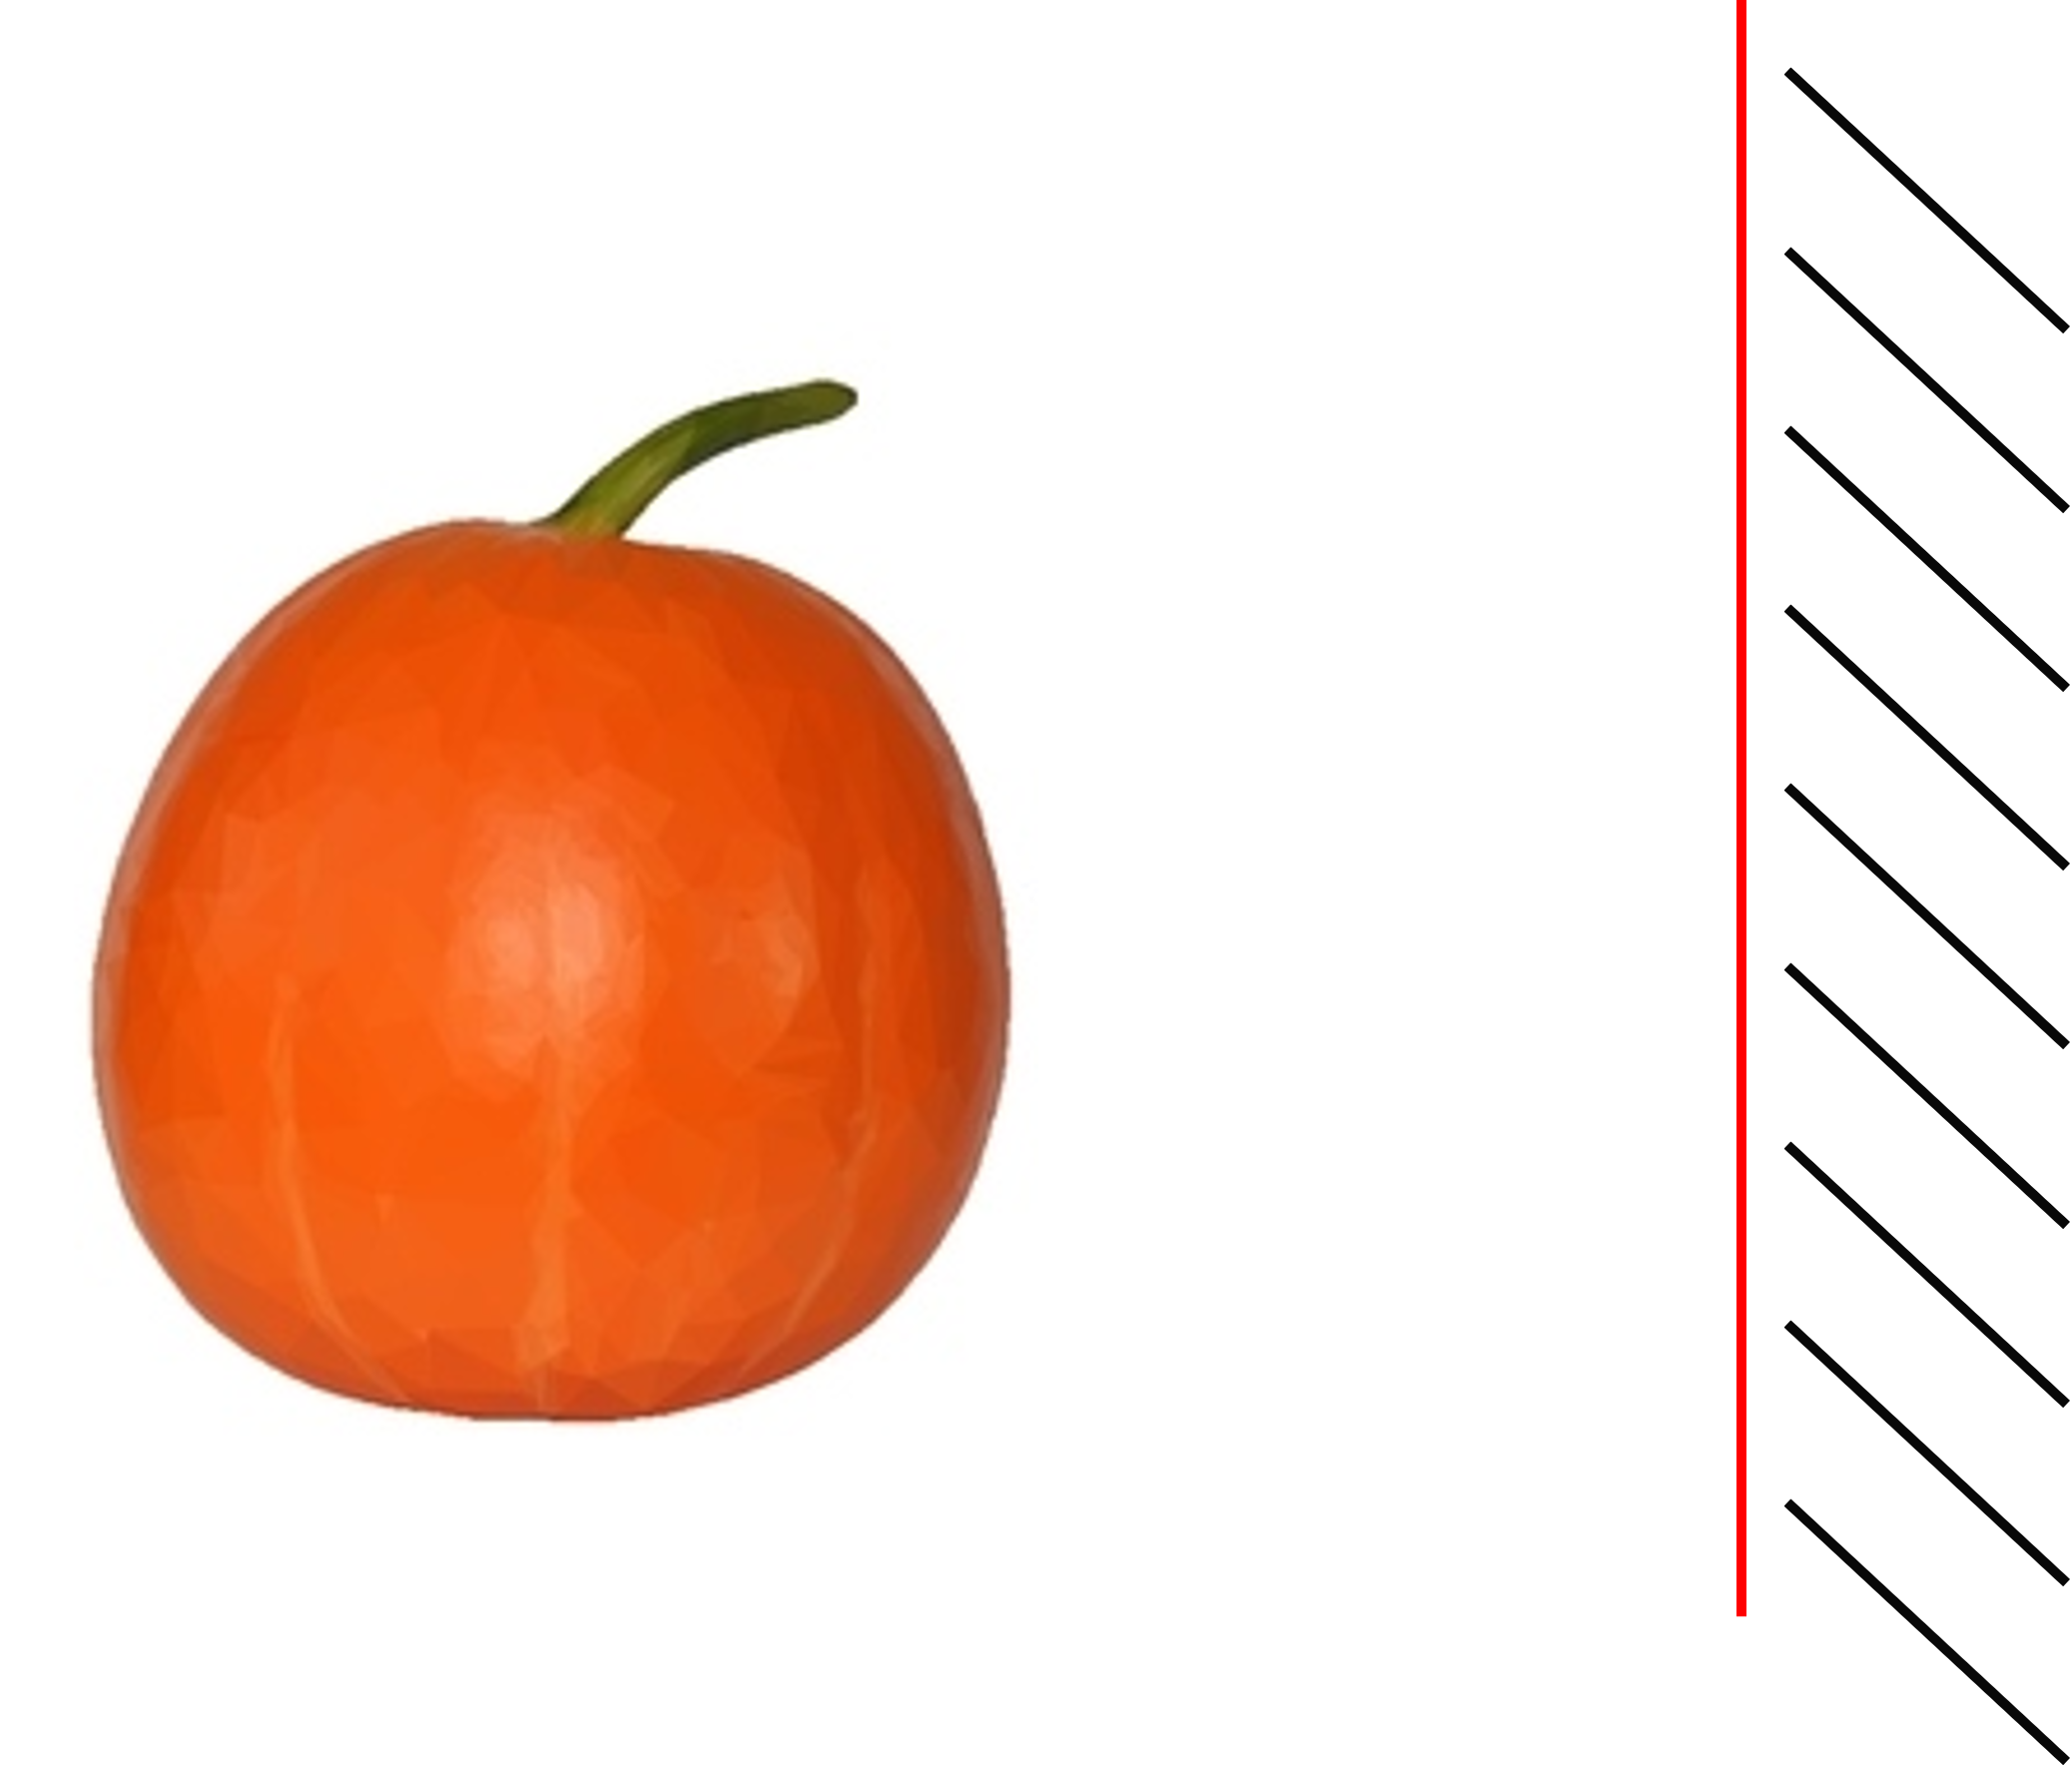
\includegraphics[width=170pt,height=110pt]{C6M14 - DT - Q3.png}},
  optionA={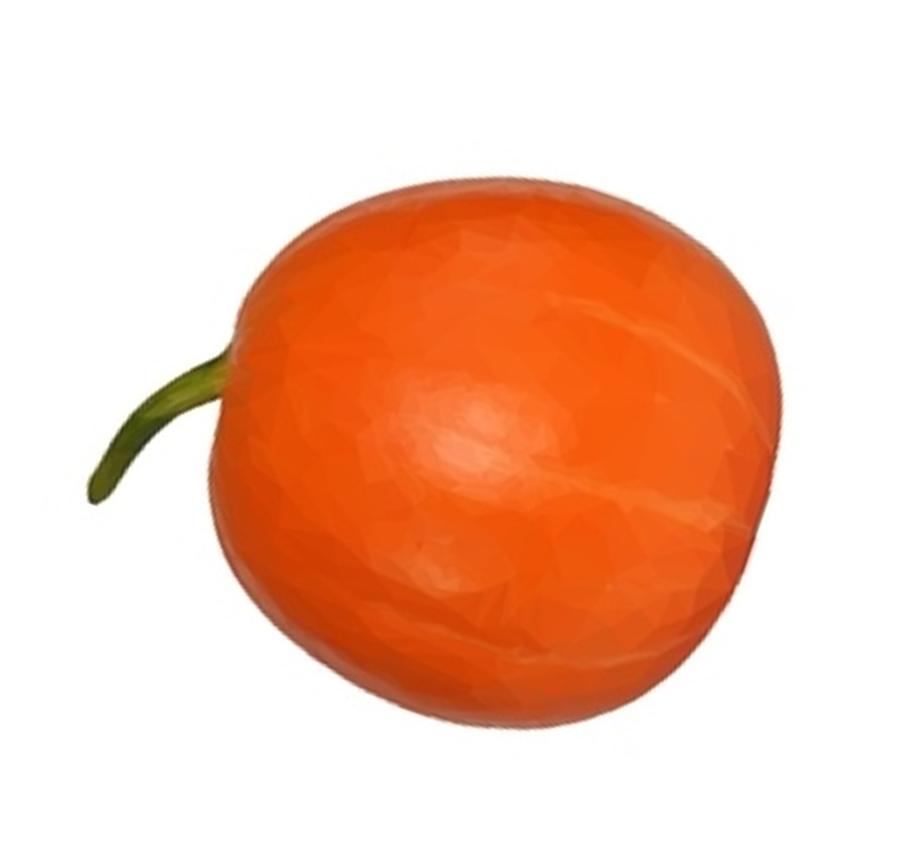
\includegraphics[width=70pt,height=50pt]{C6M14 - DT - Q3i.png}},
  optionB={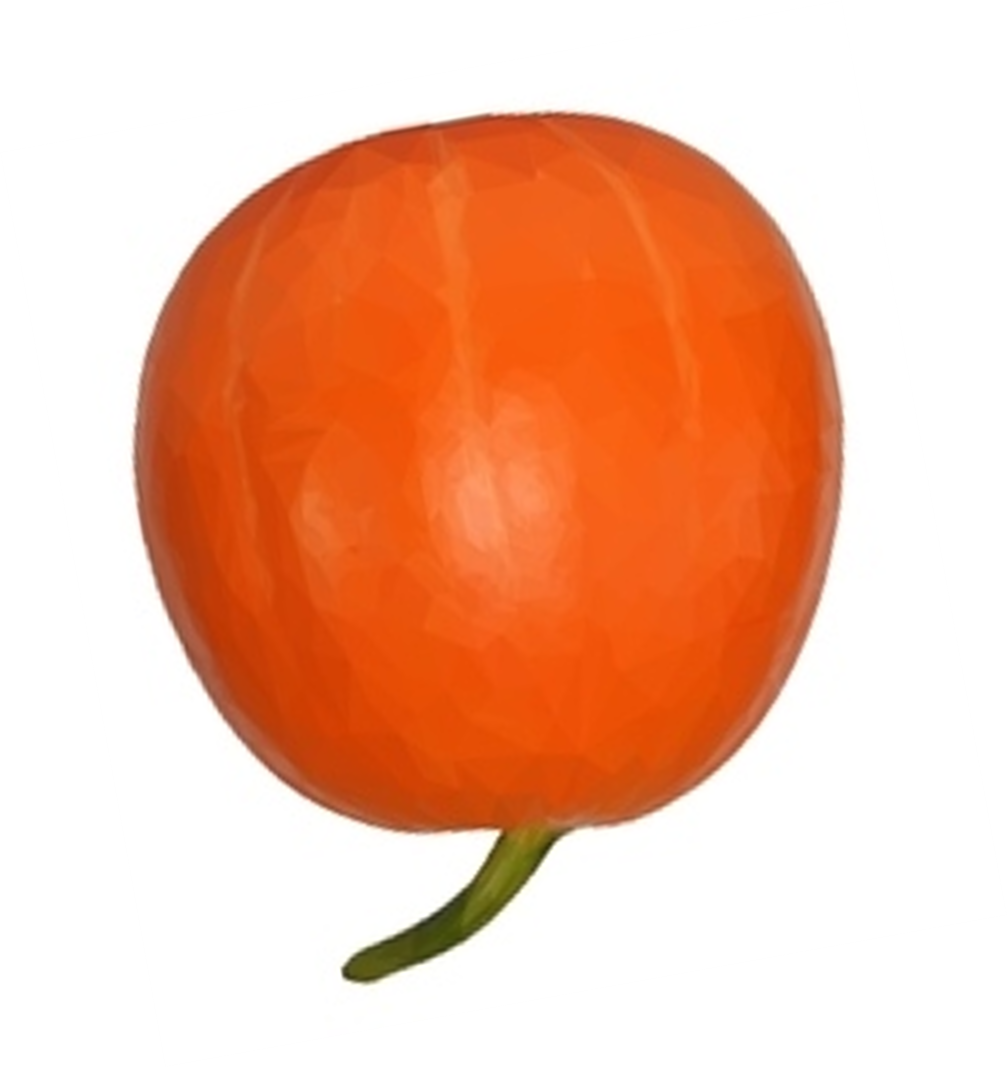
\includegraphics[width=70pt,height=50pt]{C6M14 - DT - Q3ii.png}},
  optionC={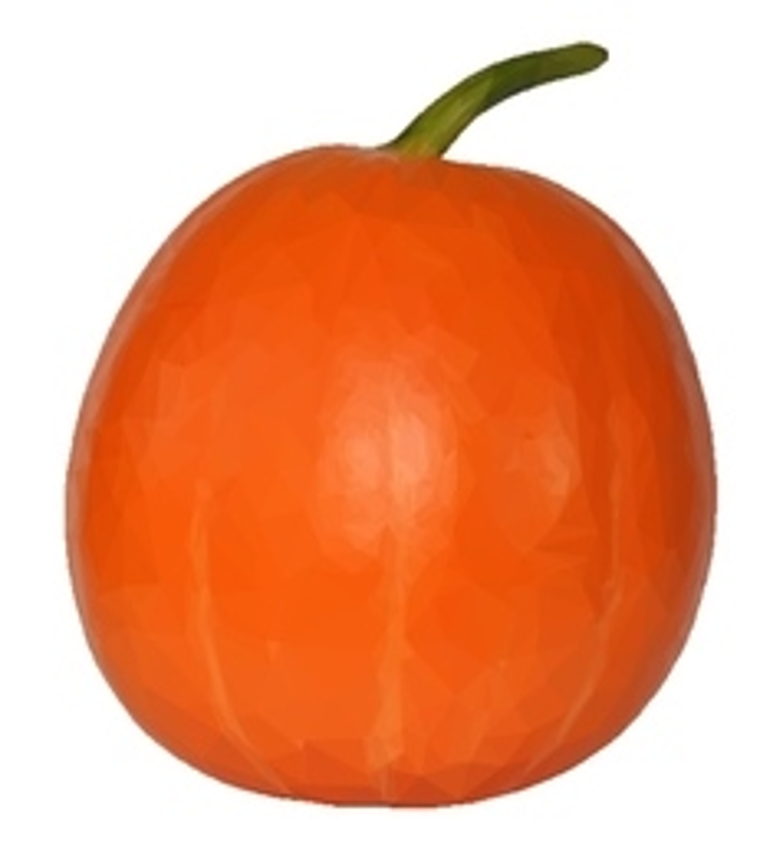
\includegraphics[width=70pt,height=50pt]{C6M14 - DT - Q3iii.png}},
  optionD={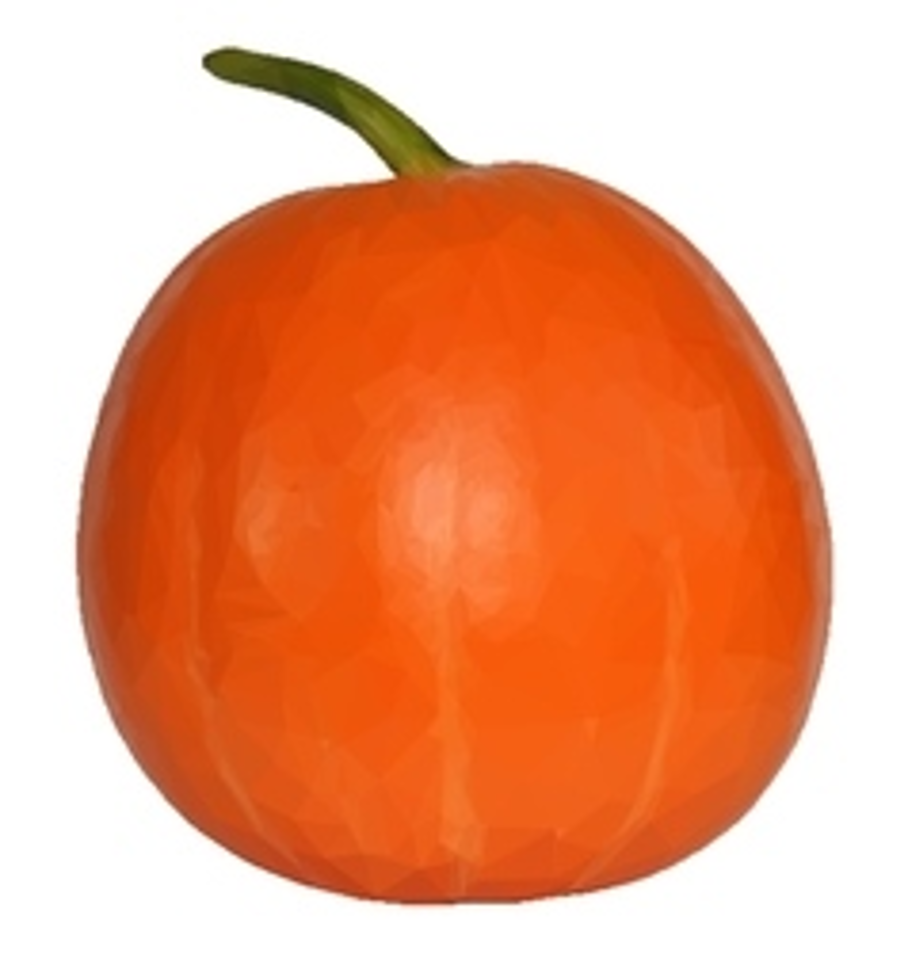
\includegraphics[width=70pt,height=50pt]{C6M14 - DT - Q3iv.png}},
  correctoption={D},}
% end-of-question

%-----------------------------------------------------------
%                        Question [ 86]
%-----------------------------------------------------------
% start-of-question
\mcqfourfour{
  questionnumber={1}, 
  questionTag={Basic arithmetic - Q1}, 
  questiontext={Add the following.\\
  \centering \includegraphics[width=600pt,height=110pt]{Basic - Q1.png}},
  optionA={14},
  optionB={12},
  optionC={68},
  optionD={6},
  correctoption={A},}
% end-of-question

%-----------------------------------------------------------
%                        Question [ 87]
%-----------------------------------------------------------

% start-of-question
\mcqfourtabletikz{
   questionnumber={2}, 
  questionTag={Basic arithmetic - Q2}, 
  questiontext={Subtract.},
  tabletikz = {
  \begin{table}[H]
  \centering
  \begin{tabular}{cccc}
   & 5 & 6 & 4  \\
   $-$ & 3 & 7 & 5\\
   \hline
   & & & \\
   \hline
    \end{tabular}
\end{table} },
   optionA={939},
  optionB={211},
  optionC={192},
  optionD={189},
  correctoption={D},
  leftmini={0.5},
  rightmini={0.4},
}
% end-of-question

%-----------------------------------------------------------
%                        Question [ 88]
%-----------------------------------------------------------
% start-of-question
\mcqfourfour{
  questionnumber={3}, 
  questionTag={Basic arithmetic - Q3}, 
  questiontext={Multiply : 1798 $\times$ 26  },
  optionA={46746},
  optionB={46744},
  optionC={46748},
  optionD={46848},
  correctoption={C},}
% end-of-question

%-----------------------------------------------------------
%                        Question [ 89]
%-----------------------------------------------------------
% start-of-question
\mcqfourfour{
  questionnumber={4}, 
  questionTag={Basic arithmetic - Q4}, 
  questiontext={Find the quotient of 1584 ÷ 3  },
  optionA={528},
  optionB={524
},
  optionC={1584},
  optionD={3},
  correctoption={A},}
% end-of-question


%-----------------------------------------------------------
%                        Question [ 90]
%-----------------------------------------------------------
% start-of-question
\mcqfourfour{
  questionnumber={5}, 
  questionTag={Basic arithmetic - Q5}, 
  questiontext={Fill in the blanks with correct symbol.\\
  \qquad ($136 + 19$)  \rule{40pt}{0.5pt}   ($173 - 28$) },
  optionA={$<$},
  optionB={$>$},
  optionC={$=$},
  optionD={None},
  correctoption={B},}
% end-of-question

%-----------------------------------------------------------
%                        Question [ 91]
%-----------------------------------------------------------
% start-of-question
\mcqfourimg{
  questionnumber={6}, 
  questionTag={Basic arithmetic - Q6}, 
  questiontext={From the figure, find the place value of the number 3.},
  imgwidth={6cm},
  imgheight={3cm},
  img={Basic - Q6.png},
  optionA={Hundreds},
  optionB={Tens},
  optionC={Thousandths},
  optionD={Ones},
  correctoption={B},
  leftmini={0.5},
  rightmini={0.5},}
% end-of-question

%-----------------------------------------------------------
%                        Question [ 92]
%-----------------------------------------------------------
% start-of-question
\mcqfourfour{
  questionnumber={7}, 
  questionTag={Basic arithmetic - Q7}, 
  questiontext={How many digits are greater than 5?\\
  \qquad 2386452662},
  optionA={4},
  optionB={5},
  optionC={10},
  optionD={1},
  correctoption={A},}
% end-of-question

%-----------------------------------------------------------
%                        Question [ 93]
%-----------------------------------------------------------
% start-of-question
\mcqfourfour{
  questionnumber={8}, 
  questionTag={Basic arithmetic - Q8}, 
  questiontext={Identify the colour of the square shape from the following.\\


\tikzset{every picture/.style={line width=0.75pt}} %set default line width to 0.75pt        

\begin{tikzpicture}[x=0.75pt,y=0.75pt,yscale=-1,xscale=1]
%uncomment if require: \path (0,300); %set diagram left start at 0, and has height of 300

%Shape: Rectangle [id:dp3316771434300363] 
\draw  [fill={rgb, 255:red, 245; green, 166; blue, 35 }  ,fill opacity=1 ] (81,62) -- (255,62) -- (255,120.92) -- (81,120.92) -- cycle ;
%Shape: Triangle [id:dp24056031036026382] 
\draw  [fill={rgb, 255:red, 240; green, 83; blue, 151 }  ,fill opacity=1 ] (375,52) -- (432,125.13) -- (318,125.13) -- cycle ;
%Shape: Square [id:dp3944643798863434] 
\draw  [fill={rgb, 255:red, 65; green, 117; blue, 5 }  ,fill opacity=1 ] (507.88,50.13) -- (583.88,50.13) -- (583.88,126.13) -- (507.88,126.13) -- cycle ;


% Text Node
\draw (54,65) node [anchor=north west][inner sep=0.75pt]   [align=left] {\textbf{i.}};
% Text Node
\draw (312,61) node [anchor=north west][inner sep=0.75pt]   [align=left] {\textbf{ii.}};
% Text Node
\draw (469,61) node [anchor=north west][inner sep=0.75pt]   [align=left] {\textbf{iii.}};


\end{tikzpicture}
},
  optionA={Violet},
  optionB={Green},
  optionC={Yellow},
  optionD={All the above},
  correctoption={B},}
% end-of-question



%-----------------------------------------------------------
%                        Question [94]
%-----------------------------------------------------------
% start-of-question
\mcqdescriptive{
  questionnumber = {   1},
  questionTag = {Critical Thinking - Q1},
  questiontext = {Rithika is fond of fancy mobile numbers. The first five digits are the descending order of digits 8, 9, 7, 0 with the lowest number repeated twice. The last five digits are the greatest five-digit number. Find the sum of the 5th and 6th numbers in the mobile number.},
  correctoption = {9},
  }
% end-of-question

%-----------------------------------------------------------
%                        Question [95]
%-----------------------------------------------------------
% start-of-question
\mcqdescriptive{
  questionnumber = {2},
  questionTag = {Critical Thinking - Q2},
  questiontext = {The bar graph depicts the total number of chocolates purchased by the group of friends. Bheem alone went and bought some additional chocolates. Calculate how many more units should be added if the total number of chocolates with Bheem is 80. \\
  \includegraphics[width=12cm, height=8cm]{CT- 2.png}
},
  correctoption = {5},
  }
% end-of-question
%-----------------------------------------------------------
%                        Question [96]
%-----------------------------------------------------------
% start-of-question
\mcqdescriptive{
  questionnumber = {3},
  questionTag = {Critical Thinking - Q3},
  questiontext = {The difference of the number of prime numbers from 0 to 50 and 60 to 100 is \rule{40pt}{0.5pt}.},
  correctoption = {7},
  }
% end-of-question


%-----------------------------------------------------------
%                        Question [97]
%-----------------------------------------------------------
% start-of-question
\mcqdescriptive{
  questionnumber = {4},
  questionTag = {Critical Thinking - Q4},
  questiontext = {Find the product of the given lines of symmetry.\\
\qquad i. 45$^\circ$ - 45$^\circ$ - 90$^\circ$ set square.\\
\qquad ii. 30$^\circ$ - 60$^\circ$ - 90$^\circ$ set square.},
  correctoption = {0},
  }
% end-of-question

%-----------------------------------------------------------
%                        Question [98]
%-----------------------------------------------------------
% start-of-question
\mcqdescriptive{
  questionnumber = {5},
  questionTag = {Critical Thinking - Q5},
  questiontext = {The length of one side of the square-shaped farm is 9 m. Rithu goes cycling around the farm in the morning and evening. Per session, she rounds the farm 11 times. Find the unit digit of the distance covered by her in a day.},
  correctoption = {2},
  }
% end-of-question

%-----------------------------------------------------------
%                        Question [99]
%-----------------------------------------------------------
% start-of-question
\mcqdescriptive{
  questionnumber = {6},
  questionTag = {Critical Thinking - Q6},
  questiontext = {Find the value of $y$ by solving the cross puzzle.\\
  \begin{table}[H]
      \centering
      \renewcommand{\arraystretch}{2}
      \begin{tabular}{ccccccccc}
           \cline{1-5}
           \multicolumn{1}{|c|}{10}& \multicolumn{1}{|c|}{+} & \multicolumn{1}{|c|}{25} & \multicolumn{1}{|c|}{=} & \multicolumn{1}{|c|}{35} &&&&\\
           \cline{1-5}
           &&&&\multicolumn{1}{|c|}{$-$} &&&&\\
           \cline{5-5}
           &&&& \multicolumn{1}{|c|}{$x$} &&&&\\
           \cline{5-5}
           &&&& \multicolumn{1}{|c|}{=} &&&&\\
           \cline{5-9}
           &&&&\multicolumn{1}{|c|}{35} &\multicolumn{1}{|c|}{$\times$} & \multicolumn{1}{|c|}{$x$}& \multicolumn{1}{|c|}{=} & \multicolumn{1}{|c|}{$y$}\\
           \cline{5-9}
      \end{tabular}
  \end{table}
  },
  correctoption = {0},
  }
% end-of-question

%-----------------------------------------------------------
%                        Question [100]
%-----------------------------------------------------------
% start-of-question
\mcqdescriptive{
  questionnumber = {7},
  questionTag = {Critical Thinking - Q7},
  questiontext = {Leo marked four points on the board and named as A, B, C, and D. He asked his friends to connect all the points in all possible ways. After connecting the points, how many lines are formed?},
  correctoption = {0},
  }
% end-of-question
%-----------------------------------------------------------
%                        Question [101]
%-----------------------------------------------------------
% start-of-question
\mcqdescriptive{
  questionnumber = {8},
  questionTag = {Critical Thinking - Q8},
  questiontext = {Vijay had a square and a rectangular piece of paper. If he tore both the papers diagonally, find the number of triangles formed with three different side lengths.},
  correctoption = {2},
  }
% end-of-question

%-----------------------------------------------------------
%                        Question [102]
%-----------------------------------------------------------
% start-of-question
\mcqdescriptive{
  questionnumber = {9},
  questionTag = {Critical Thinking - Q9},
  questiontext = {Students were assigned a task to construct a triangular prism. The triangular prism is a three-dimensional shape with two different faces. If twelve rectangular boards are given to students, how many triangular prisms can be constructed, and find the number of triangles required to construct the entire triangular prism.},
  correctoption = {8},
  }
% end-of-question

%-----------------------------------------------------------
%                        Question [103]
%-----------------------------------------------------------
% start-of-question
\mcqdescriptive{
  questionnumber = {10},
  questionTag = {Critical Thinking - Q10},
  questiontext = {If the temperature in Iceland reduces to 10$^\circ$Cand already the temperature is – 20$^\circ$C and the temperature in Delhi is 30$^\circ$C it increases 9$^\circ$C simultaneously when the temperature is reduced in Iceland. What will be the temperature in Iceland and Delhi currently also find the sum of temperature increase and decrease that happened in Delhi and Iceland.},
  correctoption = {9},
  }
% end-of-question
%-----------------------------------------------------------
%                        Question []
%-----------------------------------------------------------
% start-of-question
\mcqdescriptive{
  questionnumber = {},
  questionTag = {Critical Thinking - Q11},
  questiontext = {},
  correctoption = {},
  }
% end-of-question

%-----------------------------------------------------------
%                        Question []
%-----------------------------------------------------------
% start-of-question
\mcqdescriptive{
  questionnumber = {},
  questionTag = {Critical Thinking - Q12},
  questiontext = {},
  correctoption = {},
  }
% end-of-question

%-----------------------------------------------------------
%                        Question []
%-----------------------------------------------------------
% start-of-question
\mcqdescriptive{
  questionnumber = {},
  questionTag = {Critical Thinking - Q13},
  questiontext = {},
  correctoption = {},
  }
% end-of-question
%-----------------------------------------------------------
%                        Question []
%-----------------------------------------------------------
% start-of-question
\mcqdescriptive{
  questionnumber = {},
  questionTag = {Critical Thinking - Q14},
  questiontext = {},
  correctoption = {},
  }
% end-of-question

%-----------------------------------------------------------
%                        Question []
%-----------------------------------------------------------
% start-of-question
\mcqdescriptive{
  questionnumber = {Critical Thinking - Q15},
  questionTag = {},
  questiontext = {},
  correctoption = {},
  }
% end-of-question


\end{document}